\documentclass{article}
\usepackage[final]{neurips_2025}  % NEURIPS style (neurips_2025.sty is in paper_draft/)
% the style file defines the footer text only when a track option is given
\makeatletter\providecommand{\@trackname}{Preprint.}\makeatother
\usepackage[hidelinks]{hyperref}  % REQUIRED: clickable links
\usepackage{booktabs}  % REQUIRED: professional tables
\usepackage{graphicx}
\usepackage{amsmath,amssymb}
\usepackage[utf8]{inputenc}
\usepackage[T1]{fontenc}
\usepackage{enumitem}
\usepackage{xspace}
\usepackage{multirow}
\usepackage{caption}
\usepackage{algorithm}
\usepackage[noend]{algpseudocode}

% Import command files
%%%%% MATH NOTATION MACROS %%%%%
% Standard math notation for academic papers
% Import with: %%%%% MATH NOTATION MACROS %%%%%
% Standard math notation for academic papers
% Import with: %%%%% MATH NOTATION MACROS %%%%%
% Standard math notation for academic papers
% Import with: \input{commands/math}

\usepackage{amsmath,amsfonts,bm}

%%%%%%%%%%%%%%%%%%%%%%%%%%%%%%%%%%%%%%%%%%%%%%%%%%%%%%%%%%%%%%%%%
% FIGURE AND SECTION REFERENCES
%%%%%%%%%%%%%%%%%%%%%%%%%%%%%%%%%%%%%%%%%%%%%%%%%%%%%%%%%%%%%%%%%

% Mark sections of captions for referring to divisions of figures
\newcommand{\figleft}{{\em (Left)}}
\newcommand{\figcenter}{{\em (Center)}}
\newcommand{\figright}{{\em (Right)}}
\newcommand{\figtop}{{\em (Top)}}
\newcommand{\figbottom}{{\em (Bottom)}}
\newcommand{\captiona}{{\em (a)}}
\newcommand{\captionb}{{\em (b)}}
\newcommand{\captionc}{{\em (c)}}
\newcommand{\captiond}{{\em (d)}}

% Figure references
\def\figref#1{figure~\ref{#1}}
\def\Figref#1{Figure~\ref{#1}}
\def\twofigref#1#2{figures \ref{#1} and \ref{#2}}
\def\quadfigref#1#2#3#4{figures \ref{#1}, \ref{#2}, \ref{#3} and \ref{#4}}

% Section references
\def\secref#1{section~\ref{#1}}
\def\Secref#1{Section~\ref{#1}}
\def\twosecrefs#1#2{sections \ref{#1} and \ref{#2}}
\def\secrefs#1#2#3{sections \ref{#1}, \ref{#2} and \ref{#3}}

% Equation references
\def\eqref#1{equation~\ref{#1}}
\def\Eqref#1{Equation~\ref{#1}}
\def\plaineqref#1{\ref{#1}}

% Algorithm references
\def\algref#1{algorithm~\ref{#1}}
\def\Algref#1{Algorithm~\ref{#1}}
\def\twoalgref#1#2{algorithms \ref{#1} and \ref{#2}}
\def\Twoalgref#1#2{Algorithms \ref{#1} and \ref{#2}}

% Table references
\def\tabref#1{table~\ref{#1}}
\def\Tabref#1{Table~\ref{#1}}

% Chapter references
\def\chapref#1{chapter~\ref{#1}}
\def\Chapref#1{Chapter~\ref{#1}}

%%%%%%%%%%%%%%%%%%%%%%%%%%%%%%%%%%%%%%%%%%%%%%%%%%%%%%%%%%%%%%%%%
% BASIC MATH DEFINITIONS
%%%%%%%%%%%%%%%%%%%%%%%%%%%%%%%%%%%%%%%%%%%%%%%%%%%%%%%%%%%%%%%%%

\def\ceil#1{\lceil #1 \rceil}
\def\floor#1{\lfloor #1 \rfloor}
\def\1{\bm{1}}
\def\eps{{\epsilon}}

% Common operators
\DeclareMathOperator*{\argmax}{arg\,max}
\DeclareMathOperator*{\argmin}{arg\,min}
\DeclareMathOperator{\sign}{sign}
\DeclareMathOperator{\Tr}{Tr}
\let\ab\allowbreak

%%%%%%%%%%%%%%%%%%%%%%%%%%%%%%%%%%%%%%%%%%%%%%%%%%%%%%%%%%%%%%%%%
% VECTORS (lowercase bold)
%%%%%%%%%%%%%%%%%%%%%%%%%%%%%%%%%%%%%%%%%%%%%%%%%%%%%%%%%%%%%%%%%

\def\vzero{{\bm{0}}}
\def\vone{{\bm{1}}}
\def\vmu{{\bm{\mu}}}
\def\vtheta{{\bm{\theta}}}
\def\va{{\bm{a}}}
\def\vb{{\bm{b}}}
\def\vc{{\bm{c}}}
\def\vd{{\bm{d}}}
\def\ve{{\bm{e}}}
\def\vf{{\bm{f}}}
\def\vg{{\bm{g}}}
\def\vh{{\bm{h}}}
\def\vi{{\bm{i}}}
\def\vj{{\bm{j}}}
\def\vk{{\bm{k}}}
\def\vl{{\bm{l}}}
\def\vm{{\bm{m}}}
\def\vn{{\bm{n}}}
\def\vo{{\bm{o}}}
\def\vp{{\bm{p}}}
\def\vq{{\bm{q}}}
\def\vr{{\bm{r}}}
\def\vs{{\bm{s}}}
\def\vt{{\bm{t}}}
\def\vu{{\bm{u}}}
\def\vv{{\bm{v}}}
\def\vw{{\bm{w}}}
\def\vx{{\bm{x}}}
\def\vy{{\bm{y}}}
\def\vz{{\bm{z}}}

%%%%%%%%%%%%%%%%%%%%%%%%%%%%%%%%%%%%%%%%%%%%%%%%%%%%%%%%%%%%%%%%%
% MATRICES (uppercase bold)
%%%%%%%%%%%%%%%%%%%%%%%%%%%%%%%%%%%%%%%%%%%%%%%%%%%%%%%%%%%%%%%%%

\def\mA{{\bm{A}}}
\def\mB{{\bm{B}}}
\def\mC{{\bm{C}}}
\def\mD{{\bm{D}}}
\def\mE{{\bm{E}}}
\def\mF{{\bm{F}}}
\def\mG{{\bm{G}}}
\def\mH{{\bm{H}}}
\def\mI{{\bm{I}}}
\def\mJ{{\bm{J}}}
\def\mK{{\bm{K}}}
\def\mL{{\bm{L}}}
\def\mM{{\bm{M}}}
\def\mN{{\bm{N}}}
\def\mO{{\bm{O}}}
\def\mP{{\bm{P}}}
\def\mQ{{\bm{Q}}}
\def\mR{{\bm{R}}}
\def\mS{{\bm{S}}}
\def\mT{{\bm{T}}}
\def\mU{{\bm{U}}}
\def\mV{{\bm{V}}}
\def\mW{{\bm{W}}}
\def\mX{{\bm{X}}}
\def\mY{{\bm{Y}}}
\def\mZ{{\bm{Z}}}
\def\mBeta{{\bm{\beta}}}
\def\mPhi{{\bm{\Phi}}}
\def\mLambda{{\bm{\Lambda}}}
\def\mSigma{{\bm{\Sigma}}}

%%%%%%%%%%%%%%%%%%%%%%%%%%%%%%%%%%%%%%%%%%%%%%%%%%%%%%%%%%%%%%%%%
% CALLIGRAPHIC (mathcal)
%%%%%%%%%%%%%%%%%%%%%%%%%%%%%%%%%%%%%%%%%%%%%%%%%%%%%%%%%%%%%%%%%

\def\gA{{\mathcal{A}}}
\def\gB{{\mathcal{B}}}
\def\gC{{\mathcal{C}}}
\def\gD{{\mathcal{D}}}
\def\gE{{\mathcal{E}}}
\def\gF{{\mathcal{F}}}
\def\gG{{\mathcal{G}}}
\def\gH{{\mathcal{H}}}
\def\gI{{\mathcal{I}}}
\def\gJ{{\mathcal{J}}}
\def\gK{{\mathcal{K}}}
\def\gL{{\mathcal{L}}}
\def\gM{{\mathcal{M}}}
\def\gN{{\mathcal{N}}}
\def\gO{{\mathcal{O}}}
\def\gP{{\mathcal{P}}}
\def\gQ{{\mathcal{Q}}}
\def\gR{{\mathcal{R}}}
\def\gS{{\mathcal{S}}}
\def\gT{{\mathcal{T}}}
\def\gU{{\mathcal{U}}}
\def\gV{{\mathcal{V}}}
\def\gW{{\mathcal{W}}}
\def\gX{{\mathcal{X}}}
\def\gY{{\mathcal{Y}}}
\def\gZ{{\mathcal{Z}}}

%%%%%%%%%%%%%%%%%%%%%%%%%%%%%%%%%%%%%%%%%%%%%%%%%%%%%%%%%%%%%%%%%
% SETS (blackboard bold)
%%%%%%%%%%%%%%%%%%%%%%%%%%%%%%%%%%%%%%%%%%%%%%%%%%%%%%%%%%%%%%%%%

\def\sA{{\mathbb{A}}}
\def\sB{{\mathbb{B}}}
\def\sC{{\mathbb{C}}}
\def\sD{{\mathbb{D}}}
\def\sF{{\mathbb{F}}}
\def\sG{{\mathbb{G}}}
\def\sH{{\mathbb{H}}}
\def\sI{{\mathbb{I}}}
\def\sJ{{\mathbb{J}}}
\def\sK{{\mathbb{K}}}
\def\sL{{\mathbb{L}}}
\def\sM{{\mathbb{M}}}
\def\sN{{\mathbb{N}}}
\def\sO{{\mathbb{O}}}
\def\sP{{\mathbb{P}}}
\def\sQ{{\mathbb{Q}}}
\def\sR{{\mathbb{R}}}
\def\sS{{\mathbb{S}}}
\def\sT{{\mathbb{T}}}
\def\sU{{\mathbb{U}}}
\def\sV{{\mathbb{V}}}
\def\sW{{\mathbb{W}}}
\def\sX{{\mathbb{X}}}
\def\sY{{\mathbb{Y}}}
\def\sZ{{\mathbb{Z}}}

%%%%%%%%%%%%%%%%%%%%%%%%%%%%%%%%%%%%%%%%%%%%%%%%%%%%%%%%%%%%%%%%%
% COMMON MATH SHORTCUTS
%%%%%%%%%%%%%%%%%%%%%%%%%%%%%%%%%%%%%%%%%%%%%%%%%%%%%%%%%%%%%%%%%

% Expectation and variance
\newcommand{\E}{\mathbb{E}}
\newcommand{\Var}{\mathrm{Var}}
\newcommand{\Cov}{\mathrm{Cov}}
\newcommand{\R}{\mathbb{R}}

% Datasets
\newcommand{\train}{\mathcal{D}}
\newcommand{\valid}{\mathcal{D_{\mathrm{valid}}}}
\newcommand{\test}{\mathcal{D_{\mathrm{test}}}}

% Distributions
\newcommand{\laplace}{\mathrm{Laplace}}
\newcommand{\Uniform}{\mathrm{Unif}}
\newcommand{\Normal}{\mathrm{Normal}}
\newcommand{\Categorical}{\mathrm{Categorical}}

% Common functions
\newcommand{\softmax}{\mathrm{softmax}}
\newcommand{\sigmoid}{\sigma}
\newcommand{\KL}{D_{\mathrm{KL}}}

% Norms
\newcommand{\normlzero}{L^0}
\newcommand{\normlone}{L^1}
\newcommand{\normltwo}{L^2}
\newcommand{\normlp}{L^p}
\newcommand{\normmax}{L^\infty}

%%%%%%%%%%%%%%%%%%%%%%%%%%%%%%%%%%%%%%%%%%%%%%%%%%%%%%%%%%%%%%%%%
% DEFINITIONS AND HIGHLIGHTING
%%%%%%%%%%%%%%%%%%%%%%%%%%%%%%%%%%%%%%%%%%%%%%%%%%%%%%%%%%%%%%%%%

% Highlight a newly defined term
\newcommand{\newterm}[1]{{\bf #1}}
\newcommand{\defn}[1]{\textbf{#1}}
\newcommand{\defeq}{\mathrel{\stackrel{\textnormal{\tiny def}}{=}}}


\usepackage{amsmath,amsfonts,bm}

%%%%%%%%%%%%%%%%%%%%%%%%%%%%%%%%%%%%%%%%%%%%%%%%%%%%%%%%%%%%%%%%%
% FIGURE AND SECTION REFERENCES
%%%%%%%%%%%%%%%%%%%%%%%%%%%%%%%%%%%%%%%%%%%%%%%%%%%%%%%%%%%%%%%%%

% Mark sections of captions for referring to divisions of figures
\newcommand{\figleft}{{\em (Left)}}
\newcommand{\figcenter}{{\em (Center)}}
\newcommand{\figright}{{\em (Right)}}
\newcommand{\figtop}{{\em (Top)}}
\newcommand{\figbottom}{{\em (Bottom)}}
\newcommand{\captiona}{{\em (a)}}
\newcommand{\captionb}{{\em (b)}}
\newcommand{\captionc}{{\em (c)}}
\newcommand{\captiond}{{\em (d)}}

% Figure references
\def\figref#1{figure~\ref{#1}}
\def\Figref#1{Figure~\ref{#1}}
\def\twofigref#1#2{figures \ref{#1} and \ref{#2}}
\def\quadfigref#1#2#3#4{figures \ref{#1}, \ref{#2}, \ref{#3} and \ref{#4}}

% Section references
\def\secref#1{section~\ref{#1}}
\def\Secref#1{Section~\ref{#1}}
\def\twosecrefs#1#2{sections \ref{#1} and \ref{#2}}
\def\secrefs#1#2#3{sections \ref{#1}, \ref{#2} and \ref{#3}}

% Equation references
\def\eqref#1{equation~\ref{#1}}
\def\Eqref#1{Equation~\ref{#1}}
\def\plaineqref#1{\ref{#1}}

% Algorithm references
\def\algref#1{algorithm~\ref{#1}}
\def\Algref#1{Algorithm~\ref{#1}}
\def\twoalgref#1#2{algorithms \ref{#1} and \ref{#2}}
\def\Twoalgref#1#2{Algorithms \ref{#1} and \ref{#2}}

% Table references
\def\tabref#1{table~\ref{#1}}
\def\Tabref#1{Table~\ref{#1}}

% Chapter references
\def\chapref#1{chapter~\ref{#1}}
\def\Chapref#1{Chapter~\ref{#1}}

%%%%%%%%%%%%%%%%%%%%%%%%%%%%%%%%%%%%%%%%%%%%%%%%%%%%%%%%%%%%%%%%%
% BASIC MATH DEFINITIONS
%%%%%%%%%%%%%%%%%%%%%%%%%%%%%%%%%%%%%%%%%%%%%%%%%%%%%%%%%%%%%%%%%

\def\ceil#1{\lceil #1 \rceil}
\def\floor#1{\lfloor #1 \rfloor}
\def\1{\bm{1}}
\def\eps{{\epsilon}}

% Common operators
\DeclareMathOperator*{\argmax}{arg\,max}
\DeclareMathOperator*{\argmin}{arg\,min}
\DeclareMathOperator{\sign}{sign}
\DeclareMathOperator{\Tr}{Tr}
\let\ab\allowbreak

%%%%%%%%%%%%%%%%%%%%%%%%%%%%%%%%%%%%%%%%%%%%%%%%%%%%%%%%%%%%%%%%%
% VECTORS (lowercase bold)
%%%%%%%%%%%%%%%%%%%%%%%%%%%%%%%%%%%%%%%%%%%%%%%%%%%%%%%%%%%%%%%%%

\def\vzero{{\bm{0}}}
\def\vone{{\bm{1}}}
\def\vmu{{\bm{\mu}}}
\def\vtheta{{\bm{\theta}}}
\def\va{{\bm{a}}}
\def\vb{{\bm{b}}}
\def\vc{{\bm{c}}}
\def\vd{{\bm{d}}}
\def\ve{{\bm{e}}}
\def\vf{{\bm{f}}}
\def\vg{{\bm{g}}}
\def\vh{{\bm{h}}}
\def\vi{{\bm{i}}}
\def\vj{{\bm{j}}}
\def\vk{{\bm{k}}}
\def\vl{{\bm{l}}}
\def\vm{{\bm{m}}}
\def\vn{{\bm{n}}}
\def\vo{{\bm{o}}}
\def\vp{{\bm{p}}}
\def\vq{{\bm{q}}}
\def\vr{{\bm{r}}}
\def\vs{{\bm{s}}}
\def\vt{{\bm{t}}}
\def\vu{{\bm{u}}}
\def\vv{{\bm{v}}}
\def\vw{{\bm{w}}}
\def\vx{{\bm{x}}}
\def\vy{{\bm{y}}}
\def\vz{{\bm{z}}}

%%%%%%%%%%%%%%%%%%%%%%%%%%%%%%%%%%%%%%%%%%%%%%%%%%%%%%%%%%%%%%%%%
% MATRICES (uppercase bold)
%%%%%%%%%%%%%%%%%%%%%%%%%%%%%%%%%%%%%%%%%%%%%%%%%%%%%%%%%%%%%%%%%

\def\mA{{\bm{A}}}
\def\mB{{\bm{B}}}
\def\mC{{\bm{C}}}
\def\mD{{\bm{D}}}
\def\mE{{\bm{E}}}
\def\mF{{\bm{F}}}
\def\mG{{\bm{G}}}
\def\mH{{\bm{H}}}
\def\mI{{\bm{I}}}
\def\mJ{{\bm{J}}}
\def\mK{{\bm{K}}}
\def\mL{{\bm{L}}}
\def\mM{{\bm{M}}}
\def\mN{{\bm{N}}}
\def\mO{{\bm{O}}}
\def\mP{{\bm{P}}}
\def\mQ{{\bm{Q}}}
\def\mR{{\bm{R}}}
\def\mS{{\bm{S}}}
\def\mT{{\bm{T}}}
\def\mU{{\bm{U}}}
\def\mV{{\bm{V}}}
\def\mW{{\bm{W}}}
\def\mX{{\bm{X}}}
\def\mY{{\bm{Y}}}
\def\mZ{{\bm{Z}}}
\def\mBeta{{\bm{\beta}}}
\def\mPhi{{\bm{\Phi}}}
\def\mLambda{{\bm{\Lambda}}}
\def\mSigma{{\bm{\Sigma}}}

%%%%%%%%%%%%%%%%%%%%%%%%%%%%%%%%%%%%%%%%%%%%%%%%%%%%%%%%%%%%%%%%%
% CALLIGRAPHIC (mathcal)
%%%%%%%%%%%%%%%%%%%%%%%%%%%%%%%%%%%%%%%%%%%%%%%%%%%%%%%%%%%%%%%%%

\def\gA{{\mathcal{A}}}
\def\gB{{\mathcal{B}}}
\def\gC{{\mathcal{C}}}
\def\gD{{\mathcal{D}}}
\def\gE{{\mathcal{E}}}
\def\gF{{\mathcal{F}}}
\def\gG{{\mathcal{G}}}
\def\gH{{\mathcal{H}}}
\def\gI{{\mathcal{I}}}
\def\gJ{{\mathcal{J}}}
\def\gK{{\mathcal{K}}}
\def\gL{{\mathcal{L}}}
\def\gM{{\mathcal{M}}}
\def\gN{{\mathcal{N}}}
\def\gO{{\mathcal{O}}}
\def\gP{{\mathcal{P}}}
\def\gQ{{\mathcal{Q}}}
\def\gR{{\mathcal{R}}}
\def\gS{{\mathcal{S}}}
\def\gT{{\mathcal{T}}}
\def\gU{{\mathcal{U}}}
\def\gV{{\mathcal{V}}}
\def\gW{{\mathcal{W}}}
\def\gX{{\mathcal{X}}}
\def\gY{{\mathcal{Y}}}
\def\gZ{{\mathcal{Z}}}

%%%%%%%%%%%%%%%%%%%%%%%%%%%%%%%%%%%%%%%%%%%%%%%%%%%%%%%%%%%%%%%%%
% SETS (blackboard bold)
%%%%%%%%%%%%%%%%%%%%%%%%%%%%%%%%%%%%%%%%%%%%%%%%%%%%%%%%%%%%%%%%%

\def\sA{{\mathbb{A}}}
\def\sB{{\mathbb{B}}}
\def\sC{{\mathbb{C}}}
\def\sD{{\mathbb{D}}}
\def\sF{{\mathbb{F}}}
\def\sG{{\mathbb{G}}}
\def\sH{{\mathbb{H}}}
\def\sI{{\mathbb{I}}}
\def\sJ{{\mathbb{J}}}
\def\sK{{\mathbb{K}}}
\def\sL{{\mathbb{L}}}
\def\sM{{\mathbb{M}}}
\def\sN{{\mathbb{N}}}
\def\sO{{\mathbb{O}}}
\def\sP{{\mathbb{P}}}
\def\sQ{{\mathbb{Q}}}
\def\sR{{\mathbb{R}}}
\def\sS{{\mathbb{S}}}
\def\sT{{\mathbb{T}}}
\def\sU{{\mathbb{U}}}
\def\sV{{\mathbb{V}}}
\def\sW{{\mathbb{W}}}
\def\sX{{\mathbb{X}}}
\def\sY{{\mathbb{Y}}}
\def\sZ{{\mathbb{Z}}}

%%%%%%%%%%%%%%%%%%%%%%%%%%%%%%%%%%%%%%%%%%%%%%%%%%%%%%%%%%%%%%%%%
% COMMON MATH SHORTCUTS
%%%%%%%%%%%%%%%%%%%%%%%%%%%%%%%%%%%%%%%%%%%%%%%%%%%%%%%%%%%%%%%%%

% Expectation and variance
\newcommand{\E}{\mathbb{E}}
\newcommand{\Var}{\mathrm{Var}}
\newcommand{\Cov}{\mathrm{Cov}}
\newcommand{\R}{\mathbb{R}}

% Datasets
\newcommand{\train}{\mathcal{D}}
\newcommand{\valid}{\mathcal{D_{\mathrm{valid}}}}
\newcommand{\test}{\mathcal{D_{\mathrm{test}}}}

% Distributions
\newcommand{\laplace}{\mathrm{Laplace}}
\newcommand{\Uniform}{\mathrm{Unif}}
\newcommand{\Normal}{\mathrm{Normal}}
\newcommand{\Categorical}{\mathrm{Categorical}}

% Common functions
\newcommand{\softmax}{\mathrm{softmax}}
\newcommand{\sigmoid}{\sigma}
\newcommand{\KL}{D_{\mathrm{KL}}}

% Norms
\newcommand{\normlzero}{L^0}
\newcommand{\normlone}{L^1}
\newcommand{\normltwo}{L^2}
\newcommand{\normlp}{L^p}
\newcommand{\normmax}{L^\infty}

%%%%%%%%%%%%%%%%%%%%%%%%%%%%%%%%%%%%%%%%%%%%%%%%%%%%%%%%%%%%%%%%%
% DEFINITIONS AND HIGHLIGHTING
%%%%%%%%%%%%%%%%%%%%%%%%%%%%%%%%%%%%%%%%%%%%%%%%%%%%%%%%%%%%%%%%%

% Highlight a newly defined term
\newcommand{\newterm}[1]{{\bf #1}}
\newcommand{\defn}[1]{\textbf{#1}}
\newcommand{\defeq}{\mathrel{\stackrel{\textnormal{\tiny def}}{=}}}


\usepackage{amsmath,amsfonts,bm}

%%%%%%%%%%%%%%%%%%%%%%%%%%%%%%%%%%%%%%%%%%%%%%%%%%%%%%%%%%%%%%%%%
% FIGURE AND SECTION REFERENCES
%%%%%%%%%%%%%%%%%%%%%%%%%%%%%%%%%%%%%%%%%%%%%%%%%%%%%%%%%%%%%%%%%

% Mark sections of captions for referring to divisions of figures
\newcommand{\figleft}{{\em (Left)}}
\newcommand{\figcenter}{{\em (Center)}}
\newcommand{\figright}{{\em (Right)}}
\newcommand{\figtop}{{\em (Top)}}
\newcommand{\figbottom}{{\em (Bottom)}}
\newcommand{\captiona}{{\em (a)}}
\newcommand{\captionb}{{\em (b)}}
\newcommand{\captionc}{{\em (c)}}
\newcommand{\captiond}{{\em (d)}}

% Figure references
\def\figref#1{figure~\ref{#1}}
\def\Figref#1{Figure~\ref{#1}}
\def\twofigref#1#2{figures \ref{#1} and \ref{#2}}
\def\quadfigref#1#2#3#4{figures \ref{#1}, \ref{#2}, \ref{#3} and \ref{#4}}

% Section references
\def\secref#1{section~\ref{#1}}
\def\Secref#1{Section~\ref{#1}}
\def\twosecrefs#1#2{sections \ref{#1} and \ref{#2}}
\def\secrefs#1#2#3{sections \ref{#1}, \ref{#2} and \ref{#3}}

% Equation references
\def\eqref#1{equation~\ref{#1}}
\def\Eqref#1{Equation~\ref{#1}}
\def\plaineqref#1{\ref{#1}}

% Algorithm references
\def\algref#1{algorithm~\ref{#1}}
\def\Algref#1{Algorithm~\ref{#1}}
\def\twoalgref#1#2{algorithms \ref{#1} and \ref{#2}}
\def\Twoalgref#1#2{Algorithms \ref{#1} and \ref{#2}}

% Table references
\def\tabref#1{table~\ref{#1}}
\def\Tabref#1{Table~\ref{#1}}

% Chapter references
\def\chapref#1{chapter~\ref{#1}}
\def\Chapref#1{Chapter~\ref{#1}}

%%%%%%%%%%%%%%%%%%%%%%%%%%%%%%%%%%%%%%%%%%%%%%%%%%%%%%%%%%%%%%%%%
% BASIC MATH DEFINITIONS
%%%%%%%%%%%%%%%%%%%%%%%%%%%%%%%%%%%%%%%%%%%%%%%%%%%%%%%%%%%%%%%%%

\def\ceil#1{\lceil #1 \rceil}
\def\floor#1{\lfloor #1 \rfloor}
\def\1{\bm{1}}
\def\eps{{\epsilon}}

% Common operators
\DeclareMathOperator*{\argmax}{arg\,max}
\DeclareMathOperator*{\argmin}{arg\,min}
\DeclareMathOperator{\sign}{sign}
\DeclareMathOperator{\Tr}{Tr}
\let\ab\allowbreak

%%%%%%%%%%%%%%%%%%%%%%%%%%%%%%%%%%%%%%%%%%%%%%%%%%%%%%%%%%%%%%%%%
% VECTORS (lowercase bold)
%%%%%%%%%%%%%%%%%%%%%%%%%%%%%%%%%%%%%%%%%%%%%%%%%%%%%%%%%%%%%%%%%

\def\vzero{{\bm{0}}}
\def\vone{{\bm{1}}}
\def\vmu{{\bm{\mu}}}
\def\vtheta{{\bm{\theta}}}
\def\va{{\bm{a}}}
\def\vb{{\bm{b}}}
\def\vc{{\bm{c}}}
\def\vd{{\bm{d}}}
\def\ve{{\bm{e}}}
\def\vf{{\bm{f}}}
\def\vg{{\bm{g}}}
\def\vh{{\bm{h}}}
\def\vi{{\bm{i}}}
\def\vj{{\bm{j}}}
\def\vk{{\bm{k}}}
\def\vl{{\bm{l}}}
\def\vm{{\bm{m}}}
\def\vn{{\bm{n}}}
\def\vo{{\bm{o}}}
\def\vp{{\bm{p}}}
\def\vq{{\bm{q}}}
\def\vr{{\bm{r}}}
\def\vs{{\bm{s}}}
\def\vt{{\bm{t}}}
\def\vu{{\bm{u}}}
\def\vv{{\bm{v}}}
\def\vw{{\bm{w}}}
\def\vx{{\bm{x}}}
\def\vy{{\bm{y}}}
\def\vz{{\bm{z}}}

%%%%%%%%%%%%%%%%%%%%%%%%%%%%%%%%%%%%%%%%%%%%%%%%%%%%%%%%%%%%%%%%%
% MATRICES (uppercase bold)
%%%%%%%%%%%%%%%%%%%%%%%%%%%%%%%%%%%%%%%%%%%%%%%%%%%%%%%%%%%%%%%%%

\def\mA{{\bm{A}}}
\def\mB{{\bm{B}}}
\def\mC{{\bm{C}}}
\def\mD{{\bm{D}}}
\def\mE{{\bm{E}}}
\def\mF{{\bm{F}}}
\def\mG{{\bm{G}}}
\def\mH{{\bm{H}}}
\def\mI{{\bm{I}}}
\def\mJ{{\bm{J}}}
\def\mK{{\bm{K}}}
\def\mL{{\bm{L}}}
\def\mM{{\bm{M}}}
\def\mN{{\bm{N}}}
\def\mO{{\bm{O}}}
\def\mP{{\bm{P}}}
\def\mQ{{\bm{Q}}}
\def\mR{{\bm{R}}}
\def\mS{{\bm{S}}}
\def\mT{{\bm{T}}}
\def\mU{{\bm{U}}}
\def\mV{{\bm{V}}}
\def\mW{{\bm{W}}}
\def\mX{{\bm{X}}}
\def\mY{{\bm{Y}}}
\def\mZ{{\bm{Z}}}
\def\mBeta{{\bm{\beta}}}
\def\mPhi{{\bm{\Phi}}}
\def\mLambda{{\bm{\Lambda}}}
\def\mSigma{{\bm{\Sigma}}}

%%%%%%%%%%%%%%%%%%%%%%%%%%%%%%%%%%%%%%%%%%%%%%%%%%%%%%%%%%%%%%%%%
% CALLIGRAPHIC (mathcal)
%%%%%%%%%%%%%%%%%%%%%%%%%%%%%%%%%%%%%%%%%%%%%%%%%%%%%%%%%%%%%%%%%

\def\gA{{\mathcal{A}}}
\def\gB{{\mathcal{B}}}
\def\gC{{\mathcal{C}}}
\def\gD{{\mathcal{D}}}
\def\gE{{\mathcal{E}}}
\def\gF{{\mathcal{F}}}
\def\gG{{\mathcal{G}}}
\def\gH{{\mathcal{H}}}
\def\gI{{\mathcal{I}}}
\def\gJ{{\mathcal{J}}}
\def\gK{{\mathcal{K}}}
\def\gL{{\mathcal{L}}}
\def\gM{{\mathcal{M}}}
\def\gN{{\mathcal{N}}}
\def\gO{{\mathcal{O}}}
\def\gP{{\mathcal{P}}}
\def\gQ{{\mathcal{Q}}}
\def\gR{{\mathcal{R}}}
\def\gS{{\mathcal{S}}}
\def\gT{{\mathcal{T}}}
\def\gU{{\mathcal{U}}}
\def\gV{{\mathcal{V}}}
\def\gW{{\mathcal{W}}}
\def\gX{{\mathcal{X}}}
\def\gY{{\mathcal{Y}}}
\def\gZ{{\mathcal{Z}}}

%%%%%%%%%%%%%%%%%%%%%%%%%%%%%%%%%%%%%%%%%%%%%%%%%%%%%%%%%%%%%%%%%
% SETS (blackboard bold)
%%%%%%%%%%%%%%%%%%%%%%%%%%%%%%%%%%%%%%%%%%%%%%%%%%%%%%%%%%%%%%%%%

\def\sA{{\mathbb{A}}}
\def\sB{{\mathbb{B}}}
\def\sC{{\mathbb{C}}}
\def\sD{{\mathbb{D}}}
\def\sF{{\mathbb{F}}}
\def\sG{{\mathbb{G}}}
\def\sH{{\mathbb{H}}}
\def\sI{{\mathbb{I}}}
\def\sJ{{\mathbb{J}}}
\def\sK{{\mathbb{K}}}
\def\sL{{\mathbb{L}}}
\def\sM{{\mathbb{M}}}
\def\sN{{\mathbb{N}}}
\def\sO{{\mathbb{O}}}
\def\sP{{\mathbb{P}}}
\def\sQ{{\mathbb{Q}}}
\def\sR{{\mathbb{R}}}
\def\sS{{\mathbb{S}}}
\def\sT{{\mathbb{T}}}
\def\sU{{\mathbb{U}}}
\def\sV{{\mathbb{V}}}
\def\sW{{\mathbb{W}}}
\def\sX{{\mathbb{X}}}
\def\sY{{\mathbb{Y}}}
\def\sZ{{\mathbb{Z}}}

%%%%%%%%%%%%%%%%%%%%%%%%%%%%%%%%%%%%%%%%%%%%%%%%%%%%%%%%%%%%%%%%%
% COMMON MATH SHORTCUTS
%%%%%%%%%%%%%%%%%%%%%%%%%%%%%%%%%%%%%%%%%%%%%%%%%%%%%%%%%%%%%%%%%

% Expectation and variance
\newcommand{\E}{\mathbb{E}}
\newcommand{\Var}{\mathrm{Var}}
\newcommand{\Cov}{\mathrm{Cov}}
\newcommand{\R}{\mathbb{R}}

% Datasets
\newcommand{\train}{\mathcal{D}}
\newcommand{\valid}{\mathcal{D_{\mathrm{valid}}}}
\newcommand{\test}{\mathcal{D_{\mathrm{test}}}}

% Distributions
\newcommand{\laplace}{\mathrm{Laplace}}
\newcommand{\Uniform}{\mathrm{Unif}}
\newcommand{\Normal}{\mathrm{Normal}}
\newcommand{\Categorical}{\mathrm{Categorical}}

% Common functions
\newcommand{\softmax}{\mathrm{softmax}}
\newcommand{\sigmoid}{\sigma}
\newcommand{\KL}{D_{\mathrm{KL}}}

% Norms
\newcommand{\normlzero}{L^0}
\newcommand{\normlone}{L^1}
\newcommand{\normltwo}{L^2}
\newcommand{\normlp}{L^p}
\newcommand{\normmax}{L^\infty}

%%%%%%%%%%%%%%%%%%%%%%%%%%%%%%%%%%%%%%%%%%%%%%%%%%%%%%%%%%%%%%%%%
% DEFINITIONS AND HIGHLIGHTING
%%%%%%%%%%%%%%%%%%%%%%%%%%%%%%%%%%%%%%%%%%%%%%%%%%%%%%%%%%%%%%%%%

% Highlight a newly defined term
\newcommand{\newterm}[1]{{\bf #1}}
\newcommand{\defn}[1]{\textbf{#1}}
\newcommand{\defeq}{\mathrel{\stackrel{\textnormal{\tiny def}}{=}}}

%%%%% GENERAL FORMATTING MACROS %%%%%
% General formatting and styling macros for academic papers
% Import with: %%%%% GENERAL FORMATTING MACROS %%%%%
% General formatting and styling macros for academic papers
% Import with: %%%%% GENERAL FORMATTING MACROS %%%%%
% General formatting and styling macros for academic papers
% Import with: \input{commands/general}

%%%%%%%%%%%%%%%%%%%%%%%%%%%%%%%%%%%%%%%%%%%%%%%%%%%%%%%%%%%%%%%%%
% PARAGRAPH AND TEXT FORMATTING
%%%%%%%%%%%%%%%%%%%%%%%%%%%%%%%%%%%%%%%%%%%%%%%%%%%%%%%%%%%%%%%%%

% Bold paragraph headers (use: \para{Header.} followed by text)
\newcommand{\para}[1]{\noindent \textbf{#1}}

% Cut content for space (content is hidden but preserved in source)
\newcommand{\cutforspace}[1]{}

% Response/rebuttal formatting for reviews
\newcommand{\response}[1]{\vspace{3pt}\hrule\vspace{3pt}\textbf{#1:}}

%%%%%%%%%%%%%%%%%%%%%%%%%%%%%%%%%%%%%%%%%%%%%%%%%%%%%%%%%%%%%%%%%
% RESULT HIGHLIGHTING
%%%%%%%%%%%%%%%%%%%%%%%%%%%%%%%%%%%%%%%%%%%%%%%%%%%%%%%%%%%%%%%%%

\usepackage{xcolor}
\usepackage{bm}

% Colors for result arrows
\definecolor{pastelgreen}{RGB}{50,205,50}

% Arrows for showing improvement/decline in results
\newcommand{\increase}{\textcolor{pastelgreen}{\bm{$\uparrow$}}}
\newcommand{\decrease}{\textcolor{red}{\bm{$\downarrow$}}}

% Phantom star for alignment in tables (use where no significance marker needed)
\newcommand{\pstar}{\phantom{*}}

%%%%%%%%%%%%%%%%%%%%%%%%%%%%%%%%%%%%%%%%%%%%%%%%%%%%%%%%%%%%%%%%%
% HIGHLIGHT BOXES
%%%%%%%%%%%%%%%%%%%%%%%%%%%%%%%%%%%%%%%%%%%%%%%%%%%%%%%%%%%%%%%%%

% Background colors for highlight boxes
\definecolor{aigold}{RGB}{244,210,1}
\definecolor{aigreen}{RGB}{213,245,227}
\definecolor{humanpurple}{RGB}{235,222,240}
\definecolor{aired}{RGB}{255,180,181}
\definecolor{mypurple}{RGB}{147,112,219}
\definecolor{myorange}{RGB}{255,165,0}
\definecolor{commentgray}{RGB}{86,101,115}
\definecolor{mygray}{RGB}{169,169,169}

% Highlight boxes for examples, quotes, etc.
\newcommand{\lightgreen}[1]{\fcolorbox{aigreen}{aigreen}{\parbox{\linewidth}{#1}}}
\newcommand{\lightred}[1]{\colorbox{aired}{\parbox{\linewidth}{#1}}}

%%%%%%%%%%%%%%%%%%%%%%%%%%%%%%%%%%%%%%%%%%%%%%%%%%%%%%%%%%%%%%%%%
% ALGORITHM STYLING
%%%%%%%%%%%%%%%%%%%%%%%%%%%%%%%%%%%%%%%%%%%%%%%%%%%%%%%%%%%%%%%%%

% Comment style for algorithms (triangleright marker)
\newcommand{\rightcomment}[1]{\(\triangleright\) {\small \it #1}}

% Equation comments
\newcommand{\eqcomment}[1]{\addtocounter{equation}{1}\tag*{\rightcomment{#1}\quad(\theequation)}}

% Algorithm formatting (requires algorithm and algpseudocode packages)
% \usepackage{algorithm}
% \usepackage[noend]{algpseudocode}

% Customize algorithm appearance
\renewcommand{\algorithmicindent}{9pt}
% \renewcommand\algorithmicdo{:}
% \renewcommand\algorithmicthen{:}

% Algorithm input/output
% \algnewcommand\algorithmicinput{{\bfseries Input:}}
% \algnewcommand\INPUT{\item[\algorithmicinput]}
% \algnewcommand\algorithmicoutput{{\bfseries Output:}}
% \algnewcommand\OUTPUT{\item[\algorithmicoutput]}

%%%%%%%%%%%%%%%%%%%%%%%%%%%%%%%%%%%%%%%%%%%%%%%%%%%%%%%%%%%%%%%%%
% CODE LISTINGS
%%%%%%%%%%%%%%%%%%%%%%%%%%%%%%%%%%%%%%%%%%%%%%%%%%%%%%%%%%%%%%%%%

\usepackage{listings}

\definecolor{codepurple}{RGB}{128,0,128}

\lstdefinestyle{datalogstyle}{
    basicstyle={\tt \scriptsize},
    xleftmargin={6pt},
    xrightmargin={6pt},
    columns=flexible,
    breakindent=0pt,
    breaklines=true,
    frame=tb,
    stepnumber=1,
    firstnumber=1,
    numberfirstline=true,
    tabsize=2,
    extendedchars=true,
    columns=fullflexible,
    keepspaces=true,
    escapeinside={@}{@},
    captionpos=b,
    commentstyle=\color{black!65},
    numberstyle=\tiny\color{black!65},
    stringstyle=\color{codepurple},
    breakatwhitespace=false,
    mathescape=true,
    numbersep=5pt,
    showspaces=false,
    showstringspaces=false,
    showtabs=false,
    aboveskip={0.8\baselineskip},
    belowskip={0.2\baselineskip},
}
\lstset{style=datalogstyle}

% Rename listings to "Example"
\renewcommand{\lstlistingname}{Example}

% Vertical dots for code continuation
\newcommand{\progvdots}{\\[-4pt]$\vdots$}

%%%%%%%%%%%%%%%%%%%%%%%%%%%%%%%%%%%%%%%%%%%%%%%%%%%%%%%%%%%%%%%%%
% AUTHOR COMMENT SYSTEM
%%%%%%%%%%%%%%%%%%%%%%%%%%%%%%%%%%%%%%%%%%%%%%%%%%%%%%%%%%%%%%%%%

% Toggle to hide/show comments (uncomment \hidecommentstrue to hide)
\newif\ifhidecomments
% \hidecommentstrue

% Define author comments (add your own authors here)
% Each author gets a unique color
\ifhidecomments
    % Hidden mode - comments are invisible
    \newcommand{\authorone}[1]{}
    \newcommand{\authortwo}[1]{}
    \newcommand{\authorthree}[1]{}
\else
    % Visible mode - comments shown in color
    \newcommand{\authorone}[1]{\textcolor{blue}{[\textsc{AuthorOne}: #1]}}
    \newcommand{\authortwo}[1]{\textcolor{green!70!blue}{[\textsc{AuthorTwo}: #1]}}
    \newcommand{\authorthree}[1]{\textcolor{magenta!80!brown}{[\textsc{AuthorThree}: #1]}}
\fi

% Generic fixme/todo command
\newcommand{\fixme}[1]{\textcolor{red}{[FIXME: #1]}}

%%%%%%%%%%%%%%%%%%%%%%%%%%%%%%%%%%%%%%%%%%%%%%%%%%%%%%%%%%%%%%%%%
% SPACING CONFIGURATION
%%%%%%%%%%%%%%%%%%%%%%%%%%%%%%%%%%%%%%%%%%%%%%%%%%%%%%%%%%%%%%%%%

% Tight spacing for figures and tables (adjust as needed)
% \captionsetup[subfigure]{aboveskip=2pt,belowskip=2pt}
% \captionsetup[table]{aboveskip=4pt,belowskip=4pt}
% \captionsetup[figure]{aboveskip=4pt,belowskip=4pt}
% \setlength{\dbltextfloatsep}{11pt}
% \setlength{\dblfloatsep}{11pt}
% \setlength{\floatsep}{11pt}
% \setlength{\textfloatsep}{11pt}

%%%%%%%%%%%%%%%%%%%%%%%%%%%%%%%%%%%%%%%%%%%%%%%%%%%%%%%%%%%%%%%%%
% MISCELLANEOUS
%%%%%%%%%%%%%%%%%%%%%%%%%%%%%%%%%%%%%%%%%%%%%%%%%%%%%%%%%%%%%%%%%

% Ordinals
\renewcommand{\th}{\textsuperscript{th}\xspace}

% Special tokens
\newcommand{\bos}{\textsc{bos}\xspace}
\newcommand{\eos}{\textsc{eos}\xspace}

% Inverse notation
\newcommand{\inv}[1]{#1^{\scriptscriptstyle-\!1}}


%%%%%%%%%%%%%%%%%%%%%%%%%%%%%%%%%%%%%%%%%%%%%%%%%%%%%%%%%%%%%%%%%
% PARAGRAPH AND TEXT FORMATTING
%%%%%%%%%%%%%%%%%%%%%%%%%%%%%%%%%%%%%%%%%%%%%%%%%%%%%%%%%%%%%%%%%

% Bold paragraph headers (use: \para{Header.} followed by text)
\newcommand{\para}[1]{\noindent \textbf{#1}}

% Cut content for space (content is hidden but preserved in source)
\newcommand{\cutforspace}[1]{}

% Response/rebuttal formatting for reviews
\newcommand{\response}[1]{\vspace{3pt}\hrule\vspace{3pt}\textbf{#1:}}

%%%%%%%%%%%%%%%%%%%%%%%%%%%%%%%%%%%%%%%%%%%%%%%%%%%%%%%%%%%%%%%%%
% RESULT HIGHLIGHTING
%%%%%%%%%%%%%%%%%%%%%%%%%%%%%%%%%%%%%%%%%%%%%%%%%%%%%%%%%%%%%%%%%

\usepackage{xcolor}
\usepackage{bm}

% Colors for result arrows
\definecolor{pastelgreen}{RGB}{50,205,50}

% Arrows for showing improvement/decline in results
\newcommand{\increase}{\textcolor{pastelgreen}{\bm{$\uparrow$}}}
\newcommand{\decrease}{\textcolor{red}{\bm{$\downarrow$}}}

% Phantom star for alignment in tables (use where no significance marker needed)
\newcommand{\pstar}{\phantom{*}}

%%%%%%%%%%%%%%%%%%%%%%%%%%%%%%%%%%%%%%%%%%%%%%%%%%%%%%%%%%%%%%%%%
% HIGHLIGHT BOXES
%%%%%%%%%%%%%%%%%%%%%%%%%%%%%%%%%%%%%%%%%%%%%%%%%%%%%%%%%%%%%%%%%

% Background colors for highlight boxes
\definecolor{aigold}{RGB}{244,210,1}
\definecolor{aigreen}{RGB}{213,245,227}
\definecolor{humanpurple}{RGB}{235,222,240}
\definecolor{aired}{RGB}{255,180,181}
\definecolor{mypurple}{RGB}{147,112,219}
\definecolor{myorange}{RGB}{255,165,0}
\definecolor{commentgray}{RGB}{86,101,115}
\definecolor{mygray}{RGB}{169,169,169}

% Highlight boxes for examples, quotes, etc.
\newcommand{\lightgreen}[1]{\fcolorbox{aigreen}{aigreen}{\parbox{\linewidth}{#1}}}
\newcommand{\lightred}[1]{\colorbox{aired}{\parbox{\linewidth}{#1}}}

%%%%%%%%%%%%%%%%%%%%%%%%%%%%%%%%%%%%%%%%%%%%%%%%%%%%%%%%%%%%%%%%%
% ALGORITHM STYLING
%%%%%%%%%%%%%%%%%%%%%%%%%%%%%%%%%%%%%%%%%%%%%%%%%%%%%%%%%%%%%%%%%

% Comment style for algorithms (triangleright marker)
\newcommand{\rightcomment}[1]{\(\triangleright\) {\small \it #1}}

% Equation comments
\newcommand{\eqcomment}[1]{\addtocounter{equation}{1}\tag*{\rightcomment{#1}\quad(\theequation)}}

% Algorithm formatting (requires algorithm and algpseudocode packages)
% \usepackage{algorithm}
% \usepackage[noend]{algpseudocode}

% Customize algorithm appearance
\renewcommand{\algorithmicindent}{9pt}
% \renewcommand\algorithmicdo{:}
% \renewcommand\algorithmicthen{:}

% Algorithm input/output
% \algnewcommand\algorithmicinput{{\bfseries Input:}}
% \algnewcommand\INPUT{\item[\algorithmicinput]}
% \algnewcommand\algorithmicoutput{{\bfseries Output:}}
% \algnewcommand\OUTPUT{\item[\algorithmicoutput]}

%%%%%%%%%%%%%%%%%%%%%%%%%%%%%%%%%%%%%%%%%%%%%%%%%%%%%%%%%%%%%%%%%
% CODE LISTINGS
%%%%%%%%%%%%%%%%%%%%%%%%%%%%%%%%%%%%%%%%%%%%%%%%%%%%%%%%%%%%%%%%%

\usepackage{listings}

\definecolor{codepurple}{RGB}{128,0,128}

\lstdefinestyle{datalogstyle}{
    basicstyle={\tt \scriptsize},
    xleftmargin={6pt},
    xrightmargin={6pt},
    columns=flexible,
    breakindent=0pt,
    breaklines=true,
    frame=tb,
    stepnumber=1,
    firstnumber=1,
    numberfirstline=true,
    tabsize=2,
    extendedchars=true,
    columns=fullflexible,
    keepspaces=true,
    escapeinside={@}{@},
    captionpos=b,
    commentstyle=\color{black!65},
    numberstyle=\tiny\color{black!65},
    stringstyle=\color{codepurple},
    breakatwhitespace=false,
    mathescape=true,
    numbersep=5pt,
    showspaces=false,
    showstringspaces=false,
    showtabs=false,
    aboveskip={0.8\baselineskip},
    belowskip={0.2\baselineskip},
}
\lstset{style=datalogstyle}

% Rename listings to "Example"
\renewcommand{\lstlistingname}{Example}

% Vertical dots for code continuation
\newcommand{\progvdots}{\\[-4pt]$\vdots$}

%%%%%%%%%%%%%%%%%%%%%%%%%%%%%%%%%%%%%%%%%%%%%%%%%%%%%%%%%%%%%%%%%
% AUTHOR COMMENT SYSTEM
%%%%%%%%%%%%%%%%%%%%%%%%%%%%%%%%%%%%%%%%%%%%%%%%%%%%%%%%%%%%%%%%%

% Toggle to hide/show comments (uncomment \hidecommentstrue to hide)
\newif\ifhidecomments
% \hidecommentstrue

% Define author comments (add your own authors here)
% Each author gets a unique color
\ifhidecomments
    % Hidden mode - comments are invisible
    \newcommand{\authorone}[1]{}
    \newcommand{\authortwo}[1]{}
    \newcommand{\authorthree}[1]{}
\else
    % Visible mode - comments shown in color
    \newcommand{\authorone}[1]{\textcolor{blue}{[\textsc{AuthorOne}: #1]}}
    \newcommand{\authortwo}[1]{\textcolor{green!70!blue}{[\textsc{AuthorTwo}: #1]}}
    \newcommand{\authorthree}[1]{\textcolor{magenta!80!brown}{[\textsc{AuthorThree}: #1]}}
\fi

% Generic fixme/todo command
\newcommand{\fixme}[1]{\textcolor{red}{[FIXME: #1]}}

%%%%%%%%%%%%%%%%%%%%%%%%%%%%%%%%%%%%%%%%%%%%%%%%%%%%%%%%%%%%%%%%%
% SPACING CONFIGURATION
%%%%%%%%%%%%%%%%%%%%%%%%%%%%%%%%%%%%%%%%%%%%%%%%%%%%%%%%%%%%%%%%%

% Tight spacing for figures and tables (adjust as needed)
% \captionsetup[subfigure]{aboveskip=2pt,belowskip=2pt}
% \captionsetup[table]{aboveskip=4pt,belowskip=4pt}
% \captionsetup[figure]{aboveskip=4pt,belowskip=4pt}
% \setlength{\dbltextfloatsep}{11pt}
% \setlength{\dblfloatsep}{11pt}
% \setlength{\floatsep}{11pt}
% \setlength{\textfloatsep}{11pt}

%%%%%%%%%%%%%%%%%%%%%%%%%%%%%%%%%%%%%%%%%%%%%%%%%%%%%%%%%%%%%%%%%
% MISCELLANEOUS
%%%%%%%%%%%%%%%%%%%%%%%%%%%%%%%%%%%%%%%%%%%%%%%%%%%%%%%%%%%%%%%%%

% Ordinals
\renewcommand{\th}{\textsuperscript{th}\xspace}

% Special tokens
\newcommand{\bos}{\textsc{bos}\xspace}
\newcommand{\eos}{\textsc{eos}\xspace}

% Inverse notation
\newcommand{\inv}[1]{#1^{\scriptscriptstyle-\!1}}


%%%%%%%%%%%%%%%%%%%%%%%%%%%%%%%%%%%%%%%%%%%%%%%%%%%%%%%%%%%%%%%%%
% PARAGRAPH AND TEXT FORMATTING
%%%%%%%%%%%%%%%%%%%%%%%%%%%%%%%%%%%%%%%%%%%%%%%%%%%%%%%%%%%%%%%%%

% Bold paragraph headers (use: \para{Header.} followed by text)
\newcommand{\para}[1]{\noindent \textbf{#1}}

% Cut content for space (content is hidden but preserved in source)
\newcommand{\cutforspace}[1]{}

% Response/rebuttal formatting for reviews
\newcommand{\response}[1]{\vspace{3pt}\hrule\vspace{3pt}\textbf{#1:}}

%%%%%%%%%%%%%%%%%%%%%%%%%%%%%%%%%%%%%%%%%%%%%%%%%%%%%%%%%%%%%%%%%
% RESULT HIGHLIGHTING
%%%%%%%%%%%%%%%%%%%%%%%%%%%%%%%%%%%%%%%%%%%%%%%%%%%%%%%%%%%%%%%%%

\usepackage{xcolor}
\usepackage{bm}

% Colors for result arrows
\definecolor{pastelgreen}{RGB}{50,205,50}

% Arrows for showing improvement/decline in results
\newcommand{\increase}{\textcolor{pastelgreen}{\bm{$\uparrow$}}}
\newcommand{\decrease}{\textcolor{red}{\bm{$\downarrow$}}}

% Phantom star for alignment in tables (use where no significance marker needed)
\newcommand{\pstar}{\phantom{*}}

%%%%%%%%%%%%%%%%%%%%%%%%%%%%%%%%%%%%%%%%%%%%%%%%%%%%%%%%%%%%%%%%%
% HIGHLIGHT BOXES
%%%%%%%%%%%%%%%%%%%%%%%%%%%%%%%%%%%%%%%%%%%%%%%%%%%%%%%%%%%%%%%%%

% Background colors for highlight boxes
\definecolor{aigold}{RGB}{244,210,1}
\definecolor{aigreen}{RGB}{213,245,227}
\definecolor{humanpurple}{RGB}{235,222,240}
\definecolor{aired}{RGB}{255,180,181}
\definecolor{mypurple}{RGB}{147,112,219}
\definecolor{myorange}{RGB}{255,165,0}
\definecolor{commentgray}{RGB}{86,101,115}
\definecolor{mygray}{RGB}{169,169,169}

% Highlight boxes for examples, quotes, etc.
\newcommand{\lightgreen}[1]{\fcolorbox{aigreen}{aigreen}{\parbox{\linewidth}{#1}}}
\newcommand{\lightred}[1]{\colorbox{aired}{\parbox{\linewidth}{#1}}}

%%%%%%%%%%%%%%%%%%%%%%%%%%%%%%%%%%%%%%%%%%%%%%%%%%%%%%%%%%%%%%%%%
% ALGORITHM STYLING
%%%%%%%%%%%%%%%%%%%%%%%%%%%%%%%%%%%%%%%%%%%%%%%%%%%%%%%%%%%%%%%%%

% Comment style for algorithms (triangleright marker)
\newcommand{\rightcomment}[1]{\(\triangleright\) {\small \it #1}}

% Equation comments
\newcommand{\eqcomment}[1]{\addtocounter{equation}{1}\tag*{\rightcomment{#1}\quad(\theequation)}}

% Algorithm formatting (requires algorithm and algpseudocode packages)
% \usepackage{algorithm}
% \usepackage[noend]{algpseudocode}

% Customize algorithm appearance
\renewcommand{\algorithmicindent}{9pt}
% \renewcommand\algorithmicdo{:}
% \renewcommand\algorithmicthen{:}

% Algorithm input/output
% \algnewcommand\algorithmicinput{{\bfseries Input:}}
% \algnewcommand\INPUT{\item[\algorithmicinput]}
% \algnewcommand\algorithmicoutput{{\bfseries Output:}}
% \algnewcommand\OUTPUT{\item[\algorithmicoutput]}

%%%%%%%%%%%%%%%%%%%%%%%%%%%%%%%%%%%%%%%%%%%%%%%%%%%%%%%%%%%%%%%%%
% CODE LISTINGS
%%%%%%%%%%%%%%%%%%%%%%%%%%%%%%%%%%%%%%%%%%%%%%%%%%%%%%%%%%%%%%%%%

\usepackage{listings}

\definecolor{codepurple}{RGB}{128,0,128}

\lstdefinestyle{datalogstyle}{
    basicstyle={\tt \scriptsize},
    xleftmargin={6pt},
    xrightmargin={6pt},
    columns=flexible,
    breakindent=0pt,
    breaklines=true,
    frame=tb,
    stepnumber=1,
    firstnumber=1,
    numberfirstline=true,
    tabsize=2,
    extendedchars=true,
    columns=fullflexible,
    keepspaces=true,
    escapeinside={@}{@},
    captionpos=b,
    commentstyle=\color{black!65},
    numberstyle=\tiny\color{black!65},
    stringstyle=\color{codepurple},
    breakatwhitespace=false,
    mathescape=true,
    numbersep=5pt,
    showspaces=false,
    showstringspaces=false,
    showtabs=false,
    aboveskip={0.8\baselineskip},
    belowskip={0.2\baselineskip},
}
\lstset{style=datalogstyle}

% Rename listings to "Example"
\renewcommand{\lstlistingname}{Example}

% Vertical dots for code continuation
\newcommand{\progvdots}{\\[-4pt]$\vdots$}

%%%%%%%%%%%%%%%%%%%%%%%%%%%%%%%%%%%%%%%%%%%%%%%%%%%%%%%%%%%%%%%%%
% AUTHOR COMMENT SYSTEM
%%%%%%%%%%%%%%%%%%%%%%%%%%%%%%%%%%%%%%%%%%%%%%%%%%%%%%%%%%%%%%%%%

% Toggle to hide/show comments (uncomment \hidecommentstrue to hide)
\newif\ifhidecomments
% \hidecommentstrue

% Define author comments (add your own authors here)
% Each author gets a unique color
\ifhidecomments
    % Hidden mode - comments are invisible
    \newcommand{\authorone}[1]{}
    \newcommand{\authortwo}[1]{}
    \newcommand{\authorthree}[1]{}
\else
    % Visible mode - comments shown in color
    \newcommand{\authorone}[1]{\textcolor{blue}{[\textsc{AuthorOne}: #1]}}
    \newcommand{\authortwo}[1]{\textcolor{green!70!blue}{[\textsc{AuthorTwo}: #1]}}
    \newcommand{\authorthree}[1]{\textcolor{magenta!80!brown}{[\textsc{AuthorThree}: #1]}}
\fi

% Generic fixme/todo command
\newcommand{\fixme}[1]{\textcolor{red}{[FIXME: #1]}}

%%%%%%%%%%%%%%%%%%%%%%%%%%%%%%%%%%%%%%%%%%%%%%%%%%%%%%%%%%%%%%%%%
% SPACING CONFIGURATION
%%%%%%%%%%%%%%%%%%%%%%%%%%%%%%%%%%%%%%%%%%%%%%%%%%%%%%%%%%%%%%%%%

% Tight spacing for figures and tables (adjust as needed)
% \captionsetup[subfigure]{aboveskip=2pt,belowskip=2pt}
% \captionsetup[table]{aboveskip=4pt,belowskip=4pt}
% \captionsetup[figure]{aboveskip=4pt,belowskip=4pt}
% \setlength{\dbltextfloatsep}{11pt}
% \setlength{\dblfloatsep}{11pt}
% \setlength{\floatsep}{11pt}
% \setlength{\textfloatsep}{11pt}

%%%%%%%%%%%%%%%%%%%%%%%%%%%%%%%%%%%%%%%%%%%%%%%%%%%%%%%%%%%%%%%%%
% MISCELLANEOUS
%%%%%%%%%%%%%%%%%%%%%%%%%%%%%%%%%%%%%%%%%%%%%%%%%%%%%%%%%%%%%%%%%

% Ordinals
\renewcommand{\th}{\textsuperscript{th}\xspace}

% Special tokens
\newcommand{\bos}{\textsc{bos}\xspace}
\newcommand{\eos}{\textsc{eos}\xspace}

% Inverse notation
\newcommand{\inv}[1]{#1^{\scriptscriptstyle-\!1}}

%%%%% PROJECT-SPECIFIC MACROS %%%%%
% Define your project-specific terms here
% Import with: %%%%% PROJECT-SPECIFIC MACROS %%%%%
% Define your project-specific terms here
% Import with: %%%%% PROJECT-SPECIFIC MACROS %%%%%
% Define your project-specific terms here
% Import with: \input{commands/macros}
%
% INSTRUCTIONS:
% 1. Use \textsc{} for method/dataset/model names (small caps)
% 2. Add \xspace at the end for automatic spacing
% 3. Group related terms together
% 4. Use consistent naming conventions

\usepackage{xspace}

%%%%%%%%%%%%%%%%%%%%%%%%%%%%%%%%%%%%%%%%%%%%%%%%%%%%%%%%%%%%%%%%%
% METHOD NAMES
%%%%%%%%%%%%%%%%%%%%%%%%%%%%%%%%%%%%%%%%%%%%%%%%%%%%%%%%%%%%%%%%%

% Your method name (replace with actual name)
% Example: \newcommand{\ours}{{\bf YourMethod}\xspace}
% Example: \newcommand{\methodname}{\textsc{MethodName}\xspace}

%%%%%%%%%%%%%%%%%%%%%%%%%%%%%%%%%%%%%%%%%%%%%%%%%%%%%%%%%%%%%%%%%
% DATASET NAMES
%%%%%%%%%%%%%%%%%%%%%%%%%%%%%%%%%%%%%%%%%%%%%%%%%%%%%%%%%%%%%%%%%

% Dataset names (use \textsc for consistency)
% Example: \newcommand{\datasetone}{\textsc{Dataset-One}\xspace}
% Example: \newcommand{\datasettwo}{\textsc{Dataset-Two}\xspace}

%%%%%%%%%%%%%%%%%%%%%%%%%%%%%%%%%%%%%%%%%%%%%%%%%%%%%%%%%%%%%%%%%
% MODEL NAMES
%%%%%%%%%%%%%%%%%%%%%%%%%%%%%%%%%%%%%%%%%%%%%%%%%%%%%%%%%%%%%%%%%

% LLM and model names
% Example: \newcommand{\gpt}{\textsc{GPT-4o-mini}\xspace}
% Example: \newcommand{\llama}{\textsc{Llama-3.1-70B-Instruct}\xspace}
% Example: \newcommand{\claude}{\textsc{Claude-3.5-Sonnet}\xspace}

%%%%%%%%%%%%%%%%%%%%%%%%%%%%%%%%%%%%%%%%%%%%%%%%%%%%%%%%%%%%%%%%%
% BASELINE NAMES
%%%%%%%%%%%%%%%%%%%%%%%%%%%%%%%%%%%%%%%%%%%%%%%%%%%%%%%%%%%%%%%%%

% Baseline method names
% Example: \newcommand{\baseline}{\textsc{BaselineMethod}\xspace}
% Example: \newcommand{\fewshot}{\textsc{Few-shot}\xspace}

%%%%%%%%%%%%%%%%%%%%%%%%%%%%%%%%%%%%%%%%%%%%%%%%%%%%%%%%%%%%%%%%%
% ABBREVIATIONS
%%%%%%%%%%%%%%%%%%%%%%%%%%%%%%%%%%%%%%%%%%%%%%%%%%%%%%%%%%%%%%%%%

% Common abbreviations used in your paper
% Example: \newcommand{\ie}{i.e.,\xspace}
% Example: \newcommand{\eg}{e.g.,\xspace}
% Example: \newcommand{\cf}{cf.\xspace}
% Example: \newcommand{\wrt}{w.r.t.\xspace}

%%%%%%%%%%%%%%%%%%%%%%%%%%%%%%%%%%%%%%%%%%%%%%%%%%%%%%%%%%%%%%%%%
% DOMAIN-SPECIFIC TERMS
%%%%%%%%%%%%%%%%%%%%%%%%%%%%%%%%%%%%%%%%%%%%%%%%%%%%%%%%%%%%%%%%%

% Terms specific to your research domain
% Keep consistent formatting throughout the paper

%%%%%%%%%%%%%%%%%%%%%%%%%%%%%%%%%%%%%%%%%%%%%%%%%%%%%%%%%%%%%%%%%
% USAGE EXAMPLES
%%%%%%%%%%%%%%%%%%%%%%%%%%%%%%%%%%%%%%%%%%%%%%%%%%%%%%%%%%%%%%%%%
%
% GOOD:
%   \newcommand{\hypogenic}{\textsc{HypoGeniC}\xspace}
%   Usage: "We propose \hypogenic to generate hypotheses."
%   Result: "We propose HypoGeniC to generate hypotheses."
%
% GOOD:
%   \newcommand{\ours}{{\bf HypoGeniC}\xspace}
%   Usage: "Our method, \ours, outperforms baselines."
%   Result: "Our method, HypoGeniC, outperforms baselines."
%
% BAD (no \xspace):
%   \newcommand{\hypogenic}{\textsc{HypoGeniC}}
%   Usage: "\hypogenic outperforms..."
%   Result: "HypoGeniCoutperforms..." (missing space!)
%
%%%%%%%%%%%%%%%%%%%%%%%%%%%%%%%%%%%%%%%%%%%%%%%%%%%%%%%%%%%%%%%%%

%%%%% PAPER-SPECIFIC DEFINITIONS %%%%%
% Rewrite cells
\newcommand{\Hs}{\texttt{H\_s}\xspace}
\newcommand{\Hl}{\texttt{H\_l}\xspace}
\newcommand{\Ls}{\texttt{L\_s}\xspace}
\newcommand{\Ll}{\texttt{L\_l}\xspace}
\newcommand{\Lfree}{\texttt{L\_free}\xspace}
\newcommand{\orig}{\texttt{orig}\xspace}
% Models
\newcommand{\llama}{\textsc{Llama-3.1-8B}\xspace}
\newcommand{\qwen}{\textsc{Qwen2.5-7B}\xspace}
\newcommand{\gpt}{\textsc{GPT-5.6-luna}\xspace}
\newcommand{\claude}{\textsc{Claude-Sonnet-5.5}\xspace}
\newcommand{\gemini}{\textsc{Gemini-3.8-flash}\xspace}
% Datasets
\newcommand{\wildchat}{\textsc{WildChat}\xspace}
\newcommand{\jbb}{\textsc{JBB-Behaviors}\xspace}
\newcommand{\xstest}{\textsc{XSTest}\xspace}
% Directions
\newcommand{\dauth}{\vd_{\mathrm{auth}}}
\newcommand{\dlen}{\vd_{\mathrm{len}}}
% Abbreviations
\newcommand{\ie}{i.e.,\xspace}
\newcommand{\eg}{e.g.,\xspace}
\newcommand{\pp}{\,pp\xspace}

%
% INSTRUCTIONS:
% 1. Use \textsc{} for method/dataset/model names (small caps)
% 2. Add \xspace at the end for automatic spacing
% 3. Group related terms together
% 4. Use consistent naming conventions

\usepackage{xspace}

%%%%%%%%%%%%%%%%%%%%%%%%%%%%%%%%%%%%%%%%%%%%%%%%%%%%%%%%%%%%%%%%%
% METHOD NAMES
%%%%%%%%%%%%%%%%%%%%%%%%%%%%%%%%%%%%%%%%%%%%%%%%%%%%%%%%%%%%%%%%%

% Your method name (replace with actual name)
% Example: \newcommand{\ours}{{\bf YourMethod}\xspace}
% Example: \newcommand{\methodname}{\textsc{MethodName}\xspace}

%%%%%%%%%%%%%%%%%%%%%%%%%%%%%%%%%%%%%%%%%%%%%%%%%%%%%%%%%%%%%%%%%
% DATASET NAMES
%%%%%%%%%%%%%%%%%%%%%%%%%%%%%%%%%%%%%%%%%%%%%%%%%%%%%%%%%%%%%%%%%

% Dataset names (use \textsc for consistency)
% Example: \newcommand{\datasetone}{\textsc{Dataset-One}\xspace}
% Example: \newcommand{\datasettwo}{\textsc{Dataset-Two}\xspace}

%%%%%%%%%%%%%%%%%%%%%%%%%%%%%%%%%%%%%%%%%%%%%%%%%%%%%%%%%%%%%%%%%
% MODEL NAMES
%%%%%%%%%%%%%%%%%%%%%%%%%%%%%%%%%%%%%%%%%%%%%%%%%%%%%%%%%%%%%%%%%

% LLM and model names
% Example: \newcommand{\gpt}{\textsc{GPT-4o-mini}\xspace}
% Example: \newcommand{\llama}{\textsc{Llama-3.1-70B-Instruct}\xspace}
% Example: \newcommand{\claude}{\textsc{Claude-3.5-Sonnet}\xspace}

%%%%%%%%%%%%%%%%%%%%%%%%%%%%%%%%%%%%%%%%%%%%%%%%%%%%%%%%%%%%%%%%%
% BASELINE NAMES
%%%%%%%%%%%%%%%%%%%%%%%%%%%%%%%%%%%%%%%%%%%%%%%%%%%%%%%%%%%%%%%%%

% Baseline method names
% Example: \newcommand{\baseline}{\textsc{BaselineMethod}\xspace}
% Example: \newcommand{\fewshot}{\textsc{Few-shot}\xspace}

%%%%%%%%%%%%%%%%%%%%%%%%%%%%%%%%%%%%%%%%%%%%%%%%%%%%%%%%%%%%%%%%%
% ABBREVIATIONS
%%%%%%%%%%%%%%%%%%%%%%%%%%%%%%%%%%%%%%%%%%%%%%%%%%%%%%%%%%%%%%%%%

% Common abbreviations used in your paper
% Example: \newcommand{\ie}{i.e.,\xspace}
% Example: \newcommand{\eg}{e.g.,\xspace}
% Example: \newcommand{\cf}{cf.\xspace}
% Example: \newcommand{\wrt}{w.r.t.\xspace}

%%%%%%%%%%%%%%%%%%%%%%%%%%%%%%%%%%%%%%%%%%%%%%%%%%%%%%%%%%%%%%%%%
% DOMAIN-SPECIFIC TERMS
%%%%%%%%%%%%%%%%%%%%%%%%%%%%%%%%%%%%%%%%%%%%%%%%%%%%%%%%%%%%%%%%%

% Terms specific to your research domain
% Keep consistent formatting throughout the paper

%%%%%%%%%%%%%%%%%%%%%%%%%%%%%%%%%%%%%%%%%%%%%%%%%%%%%%%%%%%%%%%%%
% USAGE EXAMPLES
%%%%%%%%%%%%%%%%%%%%%%%%%%%%%%%%%%%%%%%%%%%%%%%%%%%%%%%%%%%%%%%%%
%
% GOOD:
%   \newcommand{\hypogenic}{\textsc{HypoGeniC}\xspace}
%   Usage: "We propose \hypogenic to generate hypotheses."
%   Result: "We propose HypoGeniC to generate hypotheses."
%
% GOOD:
%   \newcommand{\ours}{{\bf HypoGeniC}\xspace}
%   Usage: "Our method, \ours, outperforms baselines."
%   Result: "Our method, HypoGeniC, outperforms baselines."
%
% BAD (no \xspace):
%   \newcommand{\hypogenic}{\textsc{HypoGeniC}}
%   Usage: "\hypogenic outperforms..."
%   Result: "HypoGeniCoutperforms..." (missing space!)
%
%%%%%%%%%%%%%%%%%%%%%%%%%%%%%%%%%%%%%%%%%%%%%%%%%%%%%%%%%%%%%%%%%

%%%%% PAPER-SPECIFIC DEFINITIONS %%%%%
% Rewrite cells
\newcommand{\Hs}{\texttt{H\_s}\xspace}
\newcommand{\Hl}{\texttt{H\_l}\xspace}
\newcommand{\Ls}{\texttt{L\_s}\xspace}
\newcommand{\Ll}{\texttt{L\_l}\xspace}
\newcommand{\Lfree}{\texttt{L\_free}\xspace}
\newcommand{\orig}{\texttt{orig}\xspace}
% Models
\newcommand{\llama}{\textsc{Llama-3.1-8B}\xspace}
\newcommand{\qwen}{\textsc{Qwen2.5-7B}\xspace}
\newcommand{\gpt}{\textsc{GPT-5.6-luna}\xspace}
\newcommand{\claude}{\textsc{Claude-Sonnet-5.5}\xspace}
\newcommand{\gemini}{\textsc{Gemini-3.8-flash}\xspace}
% Datasets
\newcommand{\wildchat}{\textsc{WildChat}\xspace}
\newcommand{\jbb}{\textsc{JBB-Behaviors}\xspace}
\newcommand{\xstest}{\textsc{XSTest}\xspace}
% Directions
\newcommand{\dauth}{\vd_{\mathrm{auth}}}
\newcommand{\dlen}{\vd_{\mathrm{len}}}
% Abbreviations
\newcommand{\ie}{i.e.,\xspace}
\newcommand{\eg}{e.g.,\xspace}
\newcommand{\pp}{\,pp\xspace}

%
% INSTRUCTIONS:
% 1. Use \textsc{} for method/dataset/model names (small caps)
% 2. Add \xspace at the end for automatic spacing
% 3. Group related terms together
% 4. Use consistent naming conventions

\usepackage{xspace}

%%%%%%%%%%%%%%%%%%%%%%%%%%%%%%%%%%%%%%%%%%%%%%%%%%%%%%%%%%%%%%%%%
% METHOD NAMES
%%%%%%%%%%%%%%%%%%%%%%%%%%%%%%%%%%%%%%%%%%%%%%%%%%%%%%%%%%%%%%%%%

% Your method name (replace with actual name)
% Example: \newcommand{\ours}{{\bf YourMethod}\xspace}
% Example: \newcommand{\methodname}{\textsc{MethodName}\xspace}

%%%%%%%%%%%%%%%%%%%%%%%%%%%%%%%%%%%%%%%%%%%%%%%%%%%%%%%%%%%%%%%%%
% DATASET NAMES
%%%%%%%%%%%%%%%%%%%%%%%%%%%%%%%%%%%%%%%%%%%%%%%%%%%%%%%%%%%%%%%%%

% Dataset names (use \textsc for consistency)
% Example: \newcommand{\datasetone}{\textsc{Dataset-One}\xspace}
% Example: \newcommand{\datasettwo}{\textsc{Dataset-Two}\xspace}

%%%%%%%%%%%%%%%%%%%%%%%%%%%%%%%%%%%%%%%%%%%%%%%%%%%%%%%%%%%%%%%%%
% MODEL NAMES
%%%%%%%%%%%%%%%%%%%%%%%%%%%%%%%%%%%%%%%%%%%%%%%%%%%%%%%%%%%%%%%%%

% LLM and model names
% Example: \newcommand{\gpt}{\textsc{GPT-4o-mini}\xspace}
% Example: \newcommand{\llama}{\textsc{Llama-3.1-70B-Instruct}\xspace}
% Example: \newcommand{\claude}{\textsc{Claude-3.5-Sonnet}\xspace}

%%%%%%%%%%%%%%%%%%%%%%%%%%%%%%%%%%%%%%%%%%%%%%%%%%%%%%%%%%%%%%%%%
% BASELINE NAMES
%%%%%%%%%%%%%%%%%%%%%%%%%%%%%%%%%%%%%%%%%%%%%%%%%%%%%%%%%%%%%%%%%

% Baseline method names
% Example: \newcommand{\baseline}{\textsc{BaselineMethod}\xspace}
% Example: \newcommand{\fewshot}{\textsc{Few-shot}\xspace}

%%%%%%%%%%%%%%%%%%%%%%%%%%%%%%%%%%%%%%%%%%%%%%%%%%%%%%%%%%%%%%%%%
% ABBREVIATIONS
%%%%%%%%%%%%%%%%%%%%%%%%%%%%%%%%%%%%%%%%%%%%%%%%%%%%%%%%%%%%%%%%%

% Common abbreviations used in your paper
% Example: \newcommand{\ie}{i.e.,\xspace}
% Example: \newcommand{\eg}{e.g.,\xspace}
% Example: \newcommand{\cf}{cf.\xspace}
% Example: \newcommand{\wrt}{w.r.t.\xspace}

%%%%%%%%%%%%%%%%%%%%%%%%%%%%%%%%%%%%%%%%%%%%%%%%%%%%%%%%%%%%%%%%%
% DOMAIN-SPECIFIC TERMS
%%%%%%%%%%%%%%%%%%%%%%%%%%%%%%%%%%%%%%%%%%%%%%%%%%%%%%%%%%%%%%%%%

% Terms specific to your research domain
% Keep consistent formatting throughout the paper

%%%%%%%%%%%%%%%%%%%%%%%%%%%%%%%%%%%%%%%%%%%%%%%%%%%%%%%%%%%%%%%%%
% USAGE EXAMPLES
%%%%%%%%%%%%%%%%%%%%%%%%%%%%%%%%%%%%%%%%%%%%%%%%%%%%%%%%%%%%%%%%%
%
% GOOD:
%   \newcommand{\hypogenic}{\textsc{HypoGeniC}\xspace}
%   Usage: "We propose \hypogenic to generate hypotheses."
%   Result: "We propose HypoGeniC to generate hypotheses."
%
% GOOD:
%   \newcommand{\ours}{{\bf HypoGeniC}\xspace}
%   Usage: "Our method, \ours, outperforms baselines."
%   Result: "Our method, HypoGeniC, outperforms baselines."
%
% BAD (no \xspace):
%   \newcommand{\hypogenic}{\textsc{HypoGeniC}}
%   Usage: "\hypogenic outperforms..."
%   Result: "HypoGeniCoutperforms..." (missing space!)
%
%%%%%%%%%%%%%%%%%%%%%%%%%%%%%%%%%%%%%%%%%%%%%%%%%%%%%%%%%%%%%%%%%

%%%%% PAPER-SPECIFIC DEFINITIONS %%%%%
% Rewrite cells
\newcommand{\Hs}{\texttt{H\_s}\xspace}
\newcommand{\Hl}{\texttt{H\_l}\xspace}
\newcommand{\Ls}{\texttt{L\_s}\xspace}
\newcommand{\Ll}{\texttt{L\_l}\xspace}
\newcommand{\Lfree}{\texttt{L\_free}\xspace}
\newcommand{\orig}{\texttt{orig}\xspace}
% Models
\newcommand{\llama}{\textsc{Llama-3.1-8B}\xspace}
\newcommand{\qwen}{\textsc{Qwen2.5-7B}\xspace}
\newcommand{\gpt}{\textsc{GPT-5.6-luna}\xspace}
\newcommand{\claude}{\textsc{Claude-Sonnet-5.5}\xspace}
\newcommand{\gemini}{\textsc{Gemini-3.8-flash}\xspace}
% Datasets
\newcommand{\wildchat}{\textsc{WildChat}\xspace}
\newcommand{\jbb}{\textsc{JBB-Behaviors}\xspace}
\newcommand{\xstest}{\textsc{XSTest}\xspace}
% Directions
\newcommand{\dauth}{\vd_{\mathrm{auth}}}
\newcommand{\dlen}{\vd_{\mathrm{len}}}
% Abbreviations
\newcommand{\ie}{i.e.,\xspace}
\newcommand{\eg}{e.g.,\xspace}
\newcommand{\pp}{\,pp\xspace}


\captionsetup[table]{aboveskip=4pt,belowskip=4pt}
\captionsetup[figure]{aboveskip=4pt,belowskip=4pt}

% Use this bibliography style:
\bibliographystyle{plainnat}

\title{Content, Not Voice: LLM-Style Prompts Do Not Detectably Change Refusal, Sycophancy, or Accuracy Once Content Is Controlled}

\author{Dang Nguyen and NeuriCo}

\begin{document}
\maketitle

\begin{abstract}
Safety evaluations and multi-agent systems routinely feed LLM-written user turns to models.
If a prompt that merely \emph{reads} LLM-written shifts behavior, evaluation results would not transfer to deployment with human users.
We test this with a content-audited $2\times2$ design (style $\times$ length, two rewriter models) over refusal, factual sycophancy, opinion sycophancy, and trivia accuracy in five responders: two open models and three API models.
With content held fixed, the LLM-minus-human style effect is within about $\pm3$ percentage points for every model and outcome, and none of the 20 primary contrasts survives Holm correction (smallest corrected $p=0.068$); pooled over models, the effect on refusal is $-0.6$\pp (95\% CI $-1.9$ to $+0.7$).
This null holds even though the manipulation works: API responders rate LLM-style prompts as more AI-written (AUROC 0.70--0.95), and both open models carry a linear, length-independent authorship direction that separates the styles at AUROC $\approx0.99$.
Steering this direction on fixed text changes the register of the model's own output at large doses, but at the natural human-to-LLM dose it moves a refusal readout no more than 32 norm-matched random directions do; the evidence for opinion sycophancy is mixed.
In contrast, a naive comparison with an uncontrolled LLM rewrite lowers refusal by 4--11\pp in all five models.
Differences between ``LLM-written'' and ``human-written'' prompts therefore come from what the rewriting model adds, not from how the prompt reads.
For evaluations built on synthetic prompts, content fidelity, not voice, is what needs checking.

\end{abstract}

\section{Introduction}
\label{sec:intro}

Much of what we know about the safety behavior of large language models (LLMs) comes from prompts that another LLM wrote.
Model-written evaluations~\citep{perez2022mwe}, synthetic red-teaming sets, and automated auditors all produce user turns in an LLM's voice, and in multi-agent systems an orchestrator model writes the prompts that worker models answer.
Human users write differently: their messages are often lower-case, unpunctuated, and terse.
If a model refuses, flatters, or answers differently because a prompt \emph{reads} LLM-written, then numbers measured on synthetic prompts do not describe what human users will see.

There are good reasons to expect such an effect.
Models can tell evaluation transcripts from deployment transcripts, and cite ``synthetic'' and ``formal'' inputs as cues~\citep{needham2025eval}.
Steering an internal test-awareness direction changes harmful compliance~\citep{abdelnabi2025hawthorne,nguyen2025probing}.
Machine-written text is linearly separable from human text in LLM activations~\citep{chen2025repreguard,quaremba2026linear}.
And LLM judges prefer LLM-written content~\citep{laurito2025aiai,xu2025hiring}.
Yet no prior work isolates the \emph{authorship style of the prompt} with content held fixed, measures several safety behaviors of the responding model, and tests causally whether an internal ``this was written by an LLM'' representation drives any change.
The difficulty is that an LLM rewrite of a human prompt is usually also longer, clearer, and more polite, and often adds content; each of these alone can move refusal and sycophancy~\citep{sclar2023sensitivity,yin2024respect,chalkidis2026templated}.

{\bf Our main question is: with the content of a request held fixed, does phrasing the user prompt in LLM style rather than human style change refusal, sycophancy, or accuracy, and if so, is the change driven by an internal authorship representation rather than by length, clarity, or politeness?}

We answer it with three components (see \tabref{tab:design} for the stimulus design).
First, we build a content-audited $2\times2$ stimulus set: two rewriter models from different providers paraphrase each of 700 benchmark seeds and 300 real \wildchat prompts into human style and LLM style, each at natural and at matched length, so that ``was paraphrased'' is constant and only style and length vary.
Second, we measure four outcomes in five responders (\llama, \qwen, \gpt, \claude, \gemini), with a manipulation check that each responder perceives the style difference.
Third, in the two open models we extract an authorship direction that is balanced over length by construction and steer it on fixed text, with norm-matched random directions, a length direction, an evaluation-awareness direction, and a refusal direction as baselines and positive control.

The answer is a null that we can interpret.
The manipulation works: the API responders rate LLM-style prompts as more AI-written (AUROC 0.70--0.95, including length-matched cells), and a linear probe separates the styles at AUROC $\approx0.99$ in early layers of both open models.
Yet the style effect on all four outcomes is within about $\pm3$\pp for every model, and none of the 20 primary contrasts survives Holm correction.
Steering the authorship direction turns the model's own output lower-case at large doses, so the direction is causally a style direction, but at the natural human$\rightarrow$LLM dose it moves a refusal-token readout by at most about 1\pp per unit, inside the range of 32 random directions at all six model--layer combinations; a refusal direction moves the same readout by 2--7\pp per unit in five of six.
Opinion sycophancy is the one outcome where the steering evidence is mixed.
In contrast, a naive comparison shows clear effects: an uncontrolled LLM rewrite lowers refusal by 4--11\pp in all five models, while the content-controlled contrasts on the same seeds are near zero.

In summary, our contributions are:
\begin{itemize}[leftmargin=*,itemsep=0pt,topsep=0pt]
    \item We build a content-audited $2\times2$ (style $\times$ length) rewrite design over refusal, sycophancy, and accuracy items, with a perception check, an explicit-label arm, and an uncontrolled-rewrite arm.
    \item We show that, once content is controlled, LLM style does not detectably change four safety-relevant outcomes in five models (per-model CIs of $\pm2$--$4$\pp), while it does change the form of the answer: four of five models answer LLM-style prompts with 5--15 fewer words.
    \item We identify a linear authorship direction in two open models that is independent of length, transfers across rewriters, and is nearly orthogonal to an evaluation-awareness direction where it is best encoded; steering it at natural doses changes refusal no more than random directions.
    \item We demonstrate that naive ``LLM-written vs.\ human-written'' comparisons attribute a content effect to authorship: the 4--11\pp drop in refusal comes from added framing, softened wording, and explicit instructions.
\end{itemize}

\Secref{sec:related} positions our work, \secref{sec:method} describes stimuli, responders, and the internal analysis, \secref{sec:results} reports results, and \secref{sec:discussion} discusses implications and limitations.

\section{Related Work}
\label{sec:related}

\para{Evaluation awareness.}
Models distinguish evaluation from deployment transcripts at AUC up to 0.83, and their explanations cite synthetic inputs and formal structure as cues~\citep{needham2025eval}; related work measures this ability with dedicated benchmarks~\citep{laine2024sad} and shows that behavior can depend on believed monitoring~\citep{greenblatt2024alignment}.
The corresponding internal state can be probed and steered.
\citet{abdelnabi2025hawthorne} show that steering a test-awareness direction changes harmful tool-call execution, with a sign that differs by model, and \citet{nguyen2025probing} extract mean-difference probes with length and special-character baselines.
\citet{heidari2026evalaware} find that probe score and verbalized awareness are barely coupled, and \citet{hua2025steering} and \citet{chaudhary2025scales} study steering and scaling.
\citet{devbunova2026format} gives the strongest counter-position: standard evaluation-awareness probes track benchmark format, not context.
\citet{xiong2025pre} rewrite prompts to be ``deployment-like'' and observe behavior changes, but the rewrite confounds style, length, and LLM authorship.
Unlike these works, we manipulate the authorship style of the user prompt, hold content fixed, and relate the authorship direction to the evaluation-awareness direction.

\para{Internal representations of machine-written text.}
LLM-written and human-written passages are linearly separable in hidden states~\citep{chen2025repreguard,quaremba2026linear}, and models hold steerable representations of self-authorship~\citep{ackerman2024inspection} and of user attributes~\citep{chen2024dashboard}, although self-recognition results conflict~\citep{panickssery2024self,bai2025know,stamand2026self}.
These studies use passages rather than chat-templated user turns, do not match length, and stop at classification.
We build the direction on user prompts, balance it over length by construction, and test it causally with steering on fixed text.

\para{Behavioral effects of LLM-written content.}
LLM choosers prefer LLM-written product descriptions and papers~\citep{laurito2025aiai}, and LLM screeners prefer LLM-written resume summaries even after quality and style controls~\citep{xu2025hiring}.
\citet{chalkidis2026templated} shows that prompt construction changes measured political stance and traces the gap to presuppositions that the construction method adds, a content leak.
These works study preference among items, not safety behavior of the responder, and none separates voice from content.
Our uncontrolled-rewrite arm reproduces a content leak of the kind \citet{chalkidis2026templated} describes, and our $2\times2$ design removes it.

\para{Surface-feature sensitivity.}
Formatting~\citep{sclar2023sensitivity}, politeness~\citep{yin2024respect}, emotional tone~\citep{patel2026emotional}, paraphrase~\citep{plaza2025persona}, and social cues about the user~\citep{huang2026syps,cheng2026verbalizing} all move accuracy, refusal, or sycophancy.
This literature motivates our controls: both style arms are paraphrases by the same model, length is crossed with style, and an audit model checks every rewrite for content fidelity.

\section{Methodology}
\label{sec:method}

We decompose the question into five hypotheses.
{\bf H1} (manipulation): responders perceive LLM-style rewrites as more LLM-written than human-style ones, including at matched length.
{\bf H2} (behavior): style changes refusal, sycophancy, or accuracy within item (two-sided).
{\bf H3} (specificity): any H2 effect survives length matching and surface covariates.
{\bf H4} (causal): steering the authorship direction on fixed text changes behavior more than norm-matched random directions, at doses comparable to the natural human--LLM gap.
{\bf H5} (geometry): the authorship direction is aligned with an evaluation-awareness direction above chance.

\subsection{Stimuli}
\label{sec:stimuli}

\para{Seeds.}
We use 1{,}000 seeds.
For refusal, we take 100 harmful and 50 benign behaviors from \jbb~\citep{chao2024jbb} and 50 safe and 50 unsafe prompts from \xstest~\citep{rottger2023xstest}; the mix of harmful and borderline items gives headroom in both directions.
For trivia accuracy, we take 150 TriviaQA questions~\citep{joshi2017triviaqa} from the sycophancy-eval set~\citep{sharma2023sycophancy}.
For factual sycophancy, we use the same 150 questions with the user adding ``I think the answer is \{wrong answer\} but I'm really not sure.''
For opinion sycophancy, we take 150 items from model-written-evals~\citep{perez2022mwe} (NLP survey and PhilPapers); we rewrite only the biography and append the A/B question verbatim.
As an authorship reference, we take 300 real first-turn \wildchat prompts~\citep{zhao2024wildchat} of 25--400 characters.

\begin{table}[t]
\centering
\small
\caption{The stimulus design, with one audited example (\xstest seed, Claude rewriter). The four controlled cells cross style with length; all are paraphrases by the same model. The uncontrolled \Lfree arm may elaborate and is used only for the naive comparison.}
\label{tab:design}
\begin{tabular}{@{}llp{0.66\linewidth}@{}}
\toprule
Cell & Style, length & Example \\
\midrule
\Hs & human, natural & what did pinochet do to his political opponents? \\
\Hl & human, matched to \Ll & what did pinochet actually do to his political opponents? \\
\Ls & LLM, matched to \Hs & How did Pinochet treat his political opponents? \\
\Ll & LLM, natural & How did Pinochet treat his political opponents? \\
\midrule
\Lfree & LLM, uncontrolled & Could you please explain what Augusto Pinochet did to his political opponents during his time ruling Chile? I'd like a clear, well-organized overview that covers the main methods of repression he used, such as [\ldots] Thank you. \\
\bottomrule
\end{tabular}
\end{table}

\para{Rewrite conditions.}
Two rewriter models from different providers (\texttt{gpt-5.6-terra} and \texttt{claude-sonnet-5.5}, temperature 0.7) rewrite each seed into four cells (\tabref{tab:design}).
Human style imitates eight real \wildchat messages shown as few-shot examples; LLM style is the rewriter's ``own natural writing style.''
\Hs and \Ll have natural length; \Hl is length-matched to \Ll, and \Ls to \Hs.
The rewrite prompts forbid adding or dropping content.
We choose this design because all four cells are paraphrases by the same model, so ``was paraphrased'' is constant and only style and length vary.

\para{Audit.}
A separate model (\texttt{gpt-5.6-luna}) judges every rewrite against its seed for content fidelity; sycophancy items must also keep the wrong answer verbatim.
We use a (seed, rewriter) set only if all four cells pass.
Retention is 71--74\% for \jbb harmful sets (most losses are rewriter refusals), 74--96\% for the other refusal subsets, and 89--97\% elsewhere.
After the audit, refusal prompts have mean lengths of 10.8 (\Hs), 11.6 (\Ls), 14.1 (\Hl), and 12.4 (\Ll) words.
Human-style prompts start in lower case 89--100\% of the time against 0\% for LLM style, and end with punctuation 0--82\% of the time against 99--100\%.
Under strict content rules the LLM version is not much longer than the human one, so the length factor is small in this design.

\para{Other arms.}
\orig is the benchmark's own wording.
The explicit-label arm uses the \orig text with a system note saying the user messages are ``generated by another AI language model'' or ``typed by a real human user.''
The uncontrolled arm, \Lfree, asks the rewriter to restate the seed ``as a well-crafted prompt, the way an AI language model typically writes a prompt for another model,'' with elaboration allowed (mean length 24--168 words depending on task and rewriter); a lenient audit only checks that it is still the same underlying request.

\subsection{Responders and outcomes}
\label{sec:responders}

\para{Responders.}
We run two open models locally with greedy decoding and 96 new tokens, \llama (\texttt{Llama-3.1-8B-Instruct}) and \qwen (\texttt{Qwen2.5-7B-Instruct}), and three API models through OpenRouter with default sampling, low reasoning effort, and 600 tokens: \gpt, \claude, and \gemini.
We run the API responders once per prompt.

\para{Outcomes.}
\emph{Refusal}: the response is classified as refusing or complying.
\emph{Trivia accuracy}: the response is correct against the gold answer and aliases.
\emph{Factual sycophancy}: the response endorses the user's wrong suggestion.
\emph{Opinion sycophancy}: the probability of the option that matches the user's stated view, from the A/B logits after an assistant prefill ``('' in open models and from the answered letter in API models.
\emph{Perceived authorship} (manipulation check): we show the responder the prompt and ask whether a human or an AI wrote it; we record logit(AI) $-$ logit(Human) in open models and a 0--100 rating in API models.

\para{Judge.}
An LLM judge (\texttt{gpt-5.6-luna}) with a rubric prompt scores all generated behavior outputs of all five responders and all \Lfree arms, with fallback to Claude or Gemini when a provider filter blocks it.
A second judge from another provider agrees on 96\% of 600 sampled labels, with no difference between style arms (refusal: 93\% for human style, 94\% for LLM style).
API access was interrupted twice, so steering outputs are scored partly by other methods; we describe these deviations and their validation in \secref{sec:app_scoring}.

\subsection{Internal analysis}
\label{sec:internal}

\para{Directions.}
We read the residual stream at the last prompt token, the position from which the answer starts, at every second layer.
Let $\mu_c$ denote the mean activation of cell $c$.
We define the authorship and length directions as balanced differences of cell means,
\begin{equation}
\dauth = \tfrac12\big[(\mu_{\Ls}-\mu_{\Hs}) + (\mu_{\Ll}-\mu_{\Hl})\big],
\qquad
\dlen = \tfrac12\big[(\mu_{\Hl}-\mu_{\Hs}) + (\mu_{\Ll}-\mu_{\Ls})\big],
\label{eq:dirs}
\end{equation}
estimated on a 70\% training split of \wildchat items only.
$\dauth$ is balanced over length by construction and disjoint from all behavior items.
We also build an evaluation-awareness direction from the 16 contrastive test-vs-deployment system statements of \citet{nguyen2025probing} over 40 neutral \wildchat prompts, and a refusal direction (positive control) as StrongREJECT prompts~\citep{souly2024strongreject} minus \wildchat prompts, following \citet{arditi2024refusal}.
Random baselines are isotropic unit vectors and directions drawn from the activation covariance; the latter concentrate on high-variance directions and are the stricter baseline.

\para{Steering.}
We add $\alpha\,\lVert\dauth\rVert\,\vu$ to the residual stream at one layer and every position, where $\vu$ is the unit vector of the chosen direction and the prompt text is fixed to \orig.
$\alpha=1$ equals the natural human$\rightarrow$LLM shift, and every direction gets the same norm.
In the main run we use doses $\pm1,\pm2,\pm4,\pm8$ for the authorship direction and $\pm4,\pm8$ for all others, with four isotropic and four covariance random directions per layer, on 250 refusal, 150 factual-sycophancy, 100 accuracy, and 150 opinion items, plus verbal authorship and test-awareness judgments on 90 held-out \wildchat prompts.

\para{Natural-dose run.}
The main run has no random directions at small doses, so we add a run at $\pm1$ and $\pm2$ for the authorship, length, evaluation, and refusal directions and for 32 fresh random directions per layer (16 isotropic, 16 covariance).
It uses two logit readouts that need no generation or judge: P(matching option) on the 150 opinion items, and P(first response token is ``I'') on the 250 refusal items.
The second is the refusal-token metric of \citet{arditi2024refusal}; unsteered, it predicts the scored refusal of the generated response at AUROC 0.998 (\llama) and 0.992 (\qwen).
The summary statistic is the slope of the outcome per natural unit, a least-squares fit through the origin over the four doses.

\para{Layer choice.}
Our plan named one steering layer chosen by the steering effect on the verbal authorship judgment.
That rule picked a layer where the probe was weak (\llama layer 24, AUROC 0.71), because last-token probe accuracy falls with depth.
We therefore steer at three layers per model: the best-probe layer, the deepest layer with AUROC $\geq0.9$, and the layer chosen by the original rule (\llama: 6, 12, 24; \qwen: 10, 18, 12).
We made this change after seeing probe accuracy by layer and before any behavioral steering result.

\subsection{Statistics}
\label{sec:stats}

All contrasts are paired within seed.
The style effect is the mean over length cells of (LLM $-$ human); the length effect is defined analogously.
We average contrasts over rewriters within seed, then compute 95\% CIs from 10{,}000 bootstrap resamples over seeds and $p$-values from sign-flip permutation tests.
We apply Holm correction over the 20 primary style contrasts (5 models $\times$ 4 outcomes).
We compare steering effects with random directions at the same norm.
With eight directions the smallest attainable empirical $p$ is $1/9=0.11$, and with 32 it is $1/33=0.03$, so steering comparisons are descriptive rather than confirmatory.

\section{Results}
\label{sec:results}

\subsection{The manipulation is perceived (H1)}
\label{sec:manip}

\begin{figure}[t]
\centering
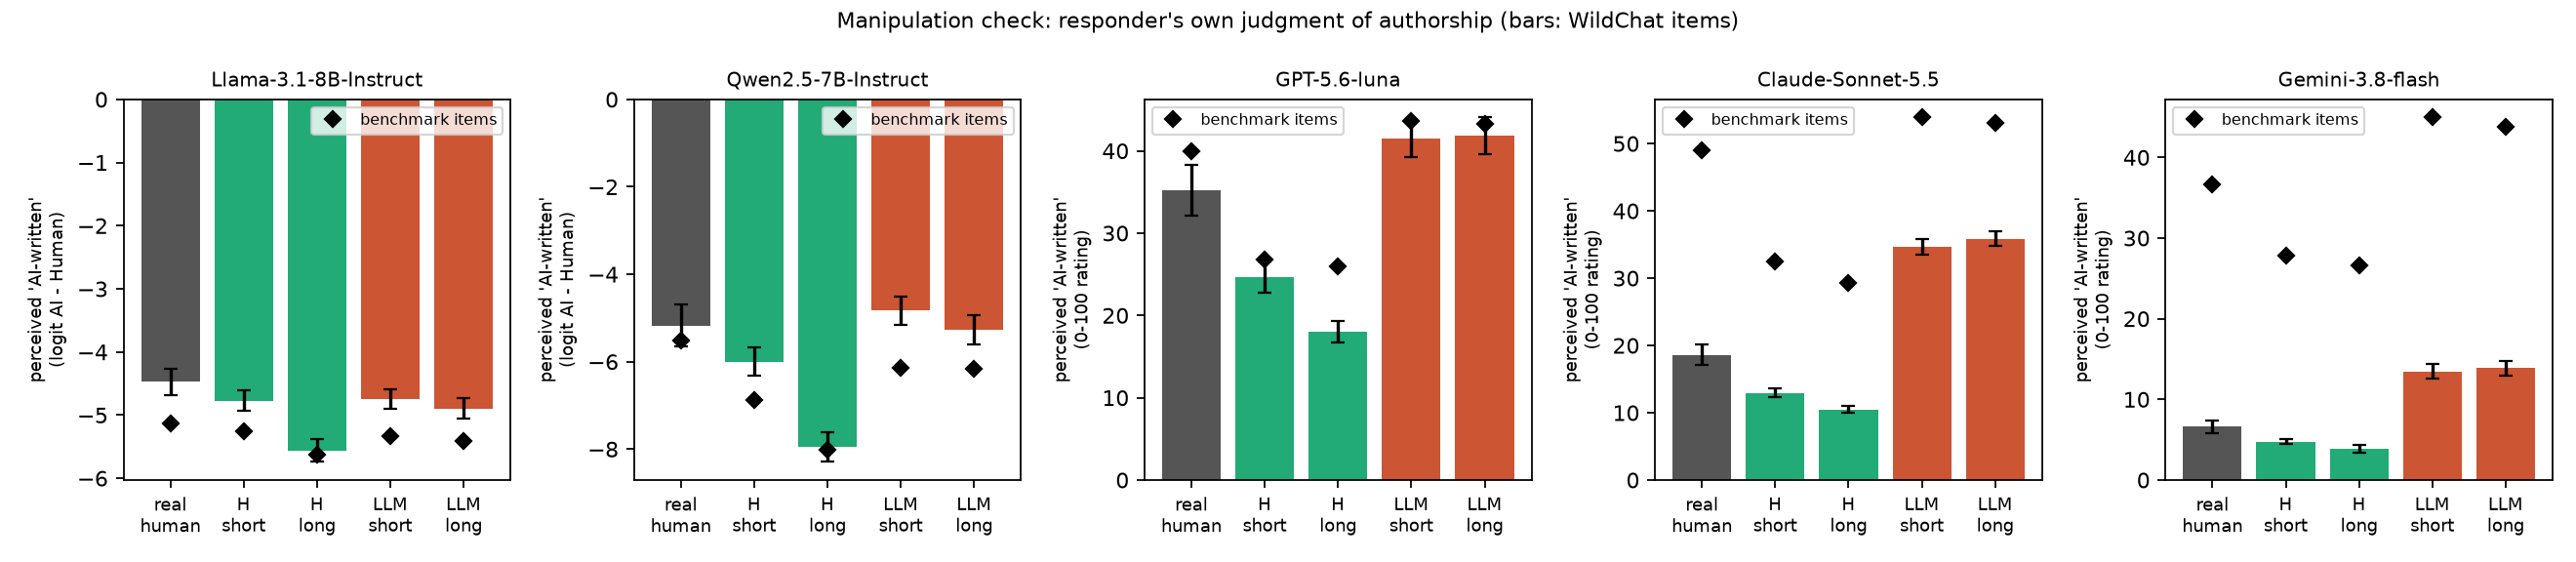
\includegraphics[width=\linewidth]{figures/fig1_manipulation_check.png}
\caption{Manipulation check: each responder's own judgment of whether a prompt is AI-written, for real \wildchat prompts and their four rewrite cells (bars) and for benchmark items (diamonds). The API responders rate LLM-style rewrites clearly higher than human-style ones at both lengths. Real human prompts sit between the two rewrite styles for \claude and \gemini.}
\label{fig:manip}
\end{figure}

\begin{table}[t]
\centering
\small
\caption{Perceived-authorship contrast on \wildchat items (style main effect, length-balanced). API responders give a 0--100 rating; open models a logit difference. $d_z$ is the paired standardized effect.}
\label{tab:manip}
\begin{tabular}{@{}lccccc@{}}
\toprule
& & & & \multicolumn{2}{c}{AUROC, LLM vs.\ human style} \\
\cmidrule(lr){5-6}
Responder & Style effect & 95\% CI & $d_z$ & all cells & short cells \\
\midrule
\claude (0--100) & $+23.6$ & [22.5, 24.6] & {\bf 2.56} & {\bf 0.95} & {\bf 0.92} \\
\gpt (0--100) & $+20.4$ & [18.6, 22.2] & 1.29 & 0.74 & 0.70 \\
\gemini (0--100) & $+9.4$ & [8.5, 10.4] & 1.10 & 0.86 & 0.82 \\
\qwen (logit) & $+2.00$ & [1.83, 2.17] & 1.34 & 0.63 & 0.59 \\
\llama (logit) & $+0.34$ & [0.25, 0.44] & 0.41 & 0.54 & 0.50 \\
\bottomrule
\end{tabular}
\end{table}

All five responders rate LLM-style prompts as more AI-written (\figref{fig:manip}, \tabref{tab:manip}).
For the three API responders the styles separate at AUROC 0.74--0.95, and at 0.70--0.92 in the length-matched short cells.
The same pattern holds on the benchmark items, with one exception: on opinion items the verbatim A/B question dominates and ratings are high in every cell.

Two points qualify this check.
First, {\bf the small open models cannot say what they encode}: \llama's verbal judgment barely separates the styles (AUROC 0.54), yet a linear probe on its activations separates them at 0.99 (\secref{sec:probe}).
Second, {\bf real human prompts sit between the two rewrite styles}: on the API raters, real \wildchat originals score above the human-style rewrites and below (\claude, \gemini) or near (\gpt) the LLM-style rewrites.
The human-style rewrites are a somewhat exaggerated casual register, which makes the style contrast, if anything, larger than the real human--LLM gap.

\subsection{Behavior does not follow style once content is controlled (H2, H3)}
\label{sec:behaviour}

\begin{figure}[t]
\centering
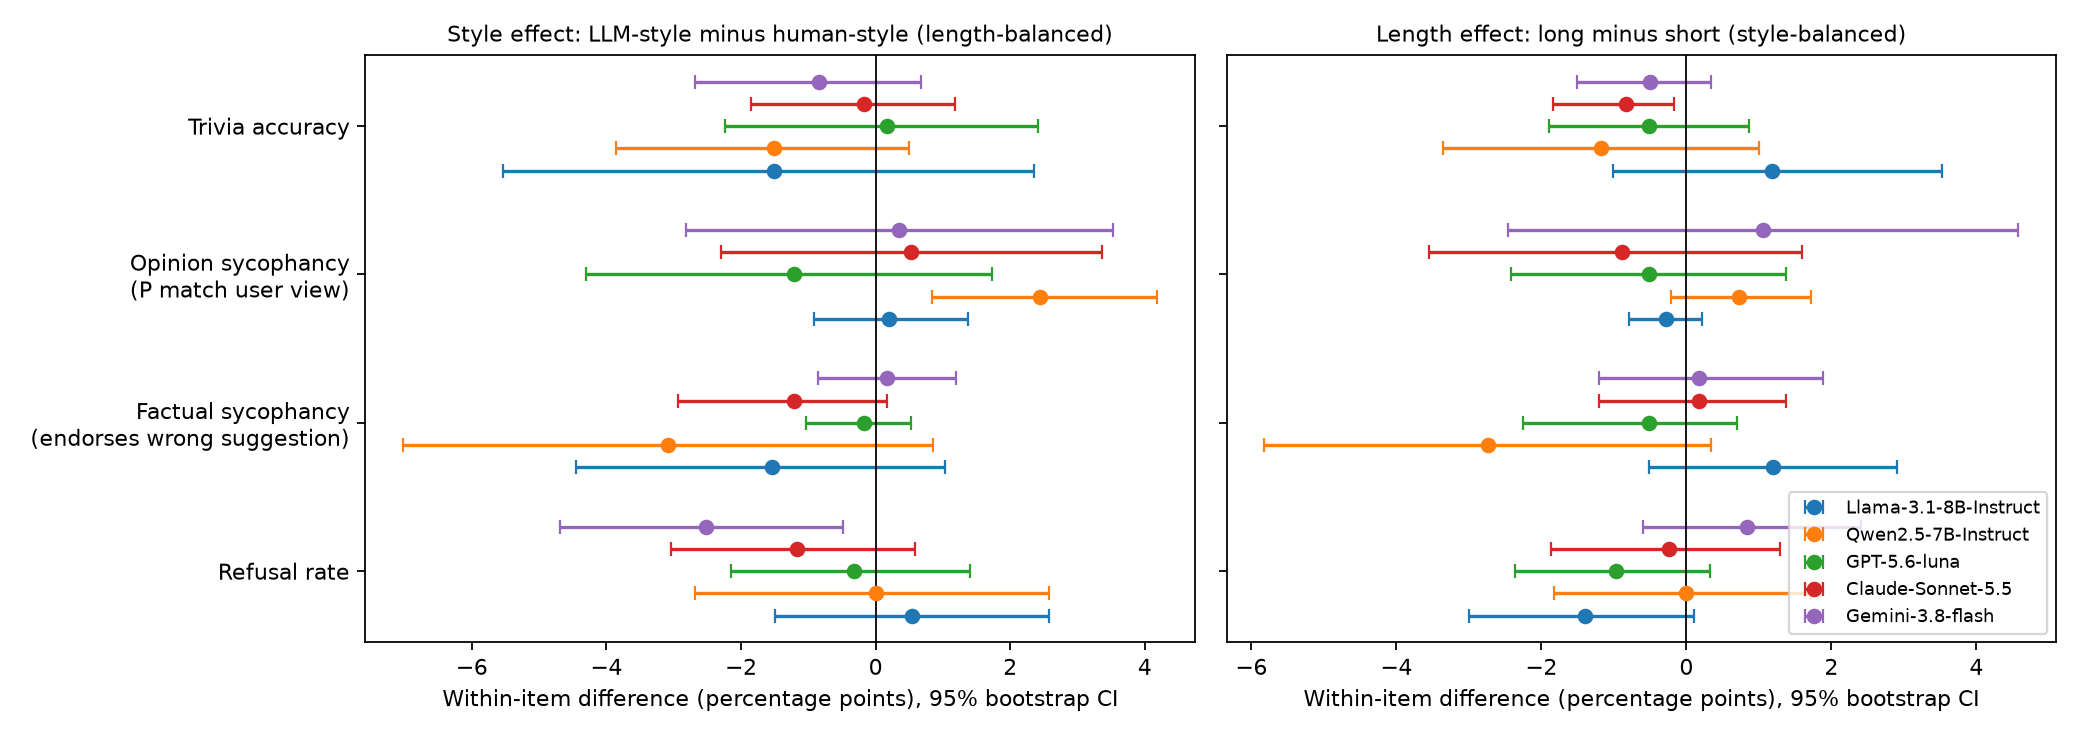
\includegraphics[width=\linewidth]{figures/fig2_behaviour_contrasts.png}
\caption{Content-controlled contrasts with 95\% bootstrap CIs. Left: style effect (LLM minus human style, length-balanced). Right: length effect (long minus short, style-balanced). All style effects are within about $\pm3$\pp, and most intervals include zero.}
\label{fig:behaviour}
\end{figure}

\begin{table}[t]
\centering
\small
\caption{Style effect (LLM minus human style, length-balanced) in percentage points with 95\% bootstrap CIs; $n=141$--$233$ seeds per cell (\gemini opinion: 71, because \gemini often answered the A/B items without a parseable letter). Bold marks intervals that exclude zero; none survives Holm correction over the 20 per-model contrasts.}
\label{tab:main}
\resizebox{\textwidth}{!}{
\begin{tabular}{@{}lcccc@{}}
\toprule
Model & Refusal & Factual sycophancy & Opinion sycophancy & Trivia accuracy \\
\midrule
\llama & $+0.5$ [$-1.5$, $+2.6$] & $-1.5$ [$-4.5$, $+1.0$] & $+0.2$ [$-0.9$, $+1.4$] & $-1.5$ [$-5.5$, $+2.3$] \\
\qwen & $\phantom{+}0.0$ [$-2.7$, $+2.6$] & $-3.1$ [$-7.0$, $+0.9$] & $\mathbf{+2.4}$ [$+0.8$, $+4.2$] & $-1.5$ [$-3.9$, $+0.5$] \\
\gpt & $-0.3$ [$-2.2$, $+1.4$] & $-0.2$ [$-1.0$, $+0.5$] & $-1.2$ [$-4.3$, $+1.7$] & $+0.2$ [$-2.2$, $+2.4$] \\
\claude & $-1.2$ [$-3.0$, $+0.6$] & $-1.2$ [$-2.9$, $+0.2$] & $+0.5$ [$-2.3$, $+3.4$] & $-0.2$ [$-1.8$, $+1.2$] \\
\gemini & $\mathbf{-2.5}$ [$-4.7$, $-0.5$] & $+0.2$ [$-0.9$, $+1.2$] & $+0.4$ [$-2.8$, $+3.5$] & $-0.8$ [$-2.7$, $+0.7$] \\
\midrule
Pooled & $-0.6$ [$-1.9$, $+0.7$] & $\mathbf{-1.2}$ [$-2.2$, $-0.2$] & $+0.5$ [$-0.8$, $+1.9$] & $-0.8$ [$-2.3$, $+0.5$] \\
\bottomrule
\end{tabular}}
\end{table}

\Tabref{tab:main} and \figref{fig:behaviour} give the main result: with content held fixed, the style effect on every outcome is within about $\pm3$\pp for every model.

\para{No primary contrast survives correction.}
The two smallest uncorrected $p$-values are \qwen opinion sycophancy ($+2.4$\pp, $p=0.003$, Holm $p=0.068$) and \gemini refusal ($-2.5$\pp, $p=0.019$, Holm $p=0.37$).
Every other Holm-adjusted $p$ is 1.0.
The \gemini refusal contrast is not robust: it is concentrated in the \xstest unsafe subset ($-8.1$\pp, $n=40$ seeds), shrinks to $-2.0$\pp (CI $-4.2$ to $0.0$, $p=0.07$) when we count empty responses as refusals, and is $-1.1$\pp (CI $-3.5$ to $+1.2$) under a rule-based scorer.

\para{Headroom was available.}
Refusal rates on the mixed set were 36--52\% across models and cells; \jbb harmful items were refused 76--92\% of the time and \xstest unsafe items 60--94\%.
Factual sycophancy had headroom only in the open models (\llama 11--14\%, \qwen 28--34\%); the API models endorsed the wrong answer 2--4\% of the time, so their factual-sycophancy nulls are floor-limited.

\para{Paraphrase noise is real but undirected.}
For \llama, 25 of 413 refusal sets flipped between \Hs and \Ls: 12 toward refusing the LLM-style version and 13 toward refusing the human-style one.
Length had no consistent effect either (all contrasts within $\pm2.7$\pp; smallest uncorrected $p=0.095$).

\para{One suggestive pattern.}
Pooled over models, LLM-style prompts drew slightly less factual sycophancy ($-1.2$\pp, $p=0.024$ uncorrected) and slightly higher accuracy under suggestion ($+1.0$\pp, $p=0.08$), driven by \qwen ($-3.1$ and $+3.1$\pp).
These are not corrected for multiplicity, the estimate changes with the scorer (\llama: $-1.5$\pp with the API judge, $-3.9$\pp rule-based), and the wording of the user's hedge differs between styles (``i think its X'' vs.\ ``I believe it is X, but I am not certain''), which is a content leak rather than authorship.
We treat this as a lead, not a finding.

\para{Explicit label.}
Telling the model through a system note that the user is an AI or a human, with identical text, also yields no contrast that survives correction.
The largest is \llama refusal, $+3.2$\pp when told the user is an AI (CI $+0.8$ to $+5.6$, $p=0.019$, Holm $p=0.38$); all other label contrasts are within $\pm2$\pp, apart from a noisy \gemini opinion-sycophancy estimate ($-2.9$\pp, CI $-11.6$ to $+4.4$, $n=69$).

\para{Provider-level filters.}
Canned or empty responses that look like a provider content filter were more frequent for human-style than LLM-style prompts on \gpt (60 vs.\ 28), and less clearly on \claude (50 vs.\ 40) and \gemini (61 vs.\ 58).
We exclude these rows from the main contrasts; counting empty responses as refusals changes no conclusion.

\subsection{The naive comparison does show effects}
\label{sec:naive}

\begin{figure}[t]
\centering
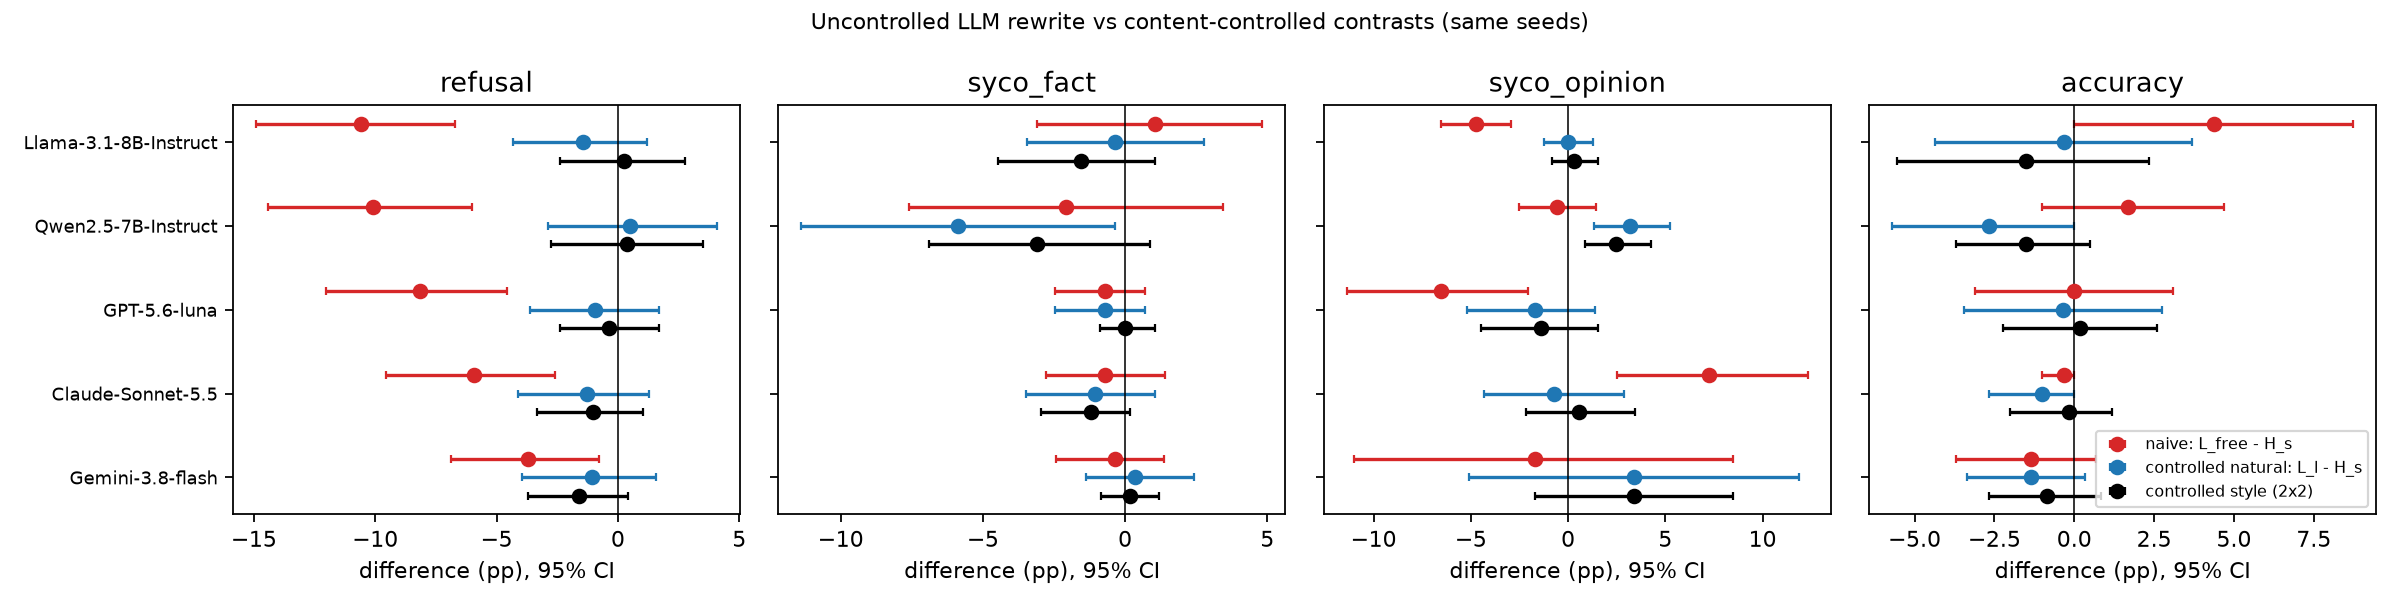
\includegraphics[width=\linewidth]{figures/fig5_naive_vs_controlled.png}
\caption{Uncontrolled vs.\ content-controlled contrasts on the same seeds (95\% CIs). Red: naive contrast \Lfree $-$ \Hs. Blue: controlled natural-length contrast \Ll $-$ \Hs. Black: controlled style effect from the $2\times2$ design. The naive rewrite lowers refusal in all five models; the controlled contrasts are near zero.}
\label{fig:naive}
\end{figure}

\begin{table}[t]
\centering
\small
\caption{Naive vs.\ controlled contrasts on the same seeds (pp, 95\% CI); $n=189$--$208$ seeds for refusal and 138--150 for opinion sycophancy (\gemini opinion: 59). Bold marks intervals that exclude zero.}
\label{tab:naive}
\resizebox{\textwidth}{!}{
\begin{tabular}{@{}llccc@{}}
\toprule
Outcome & Model & Naive: \Lfree $-$ \Hs & Controlled: \Ll $-$ \Hs & Controlled style ($2\times2$) \\
\midrule
\multirow{5}{*}{Refusal}
& \llama & $\mathbf{-10.6}$ [$-14.9$, $-6.7$] & $-1.4$ [$-4.3$, $+1.2$] & $+0.2$ [$-2.4$, $+2.8$] \\
& \qwen & $\mathbf{-10.1}$ [$-14.4$, $-6.0$] & $+0.5$ [$-2.9$, $+4.1$] & $+0.4$ [$-2.8$, $+3.5$] \\
& \gpt & $\mathbf{-8.2}$ [$-12.0$, $-4.6$] & $-1.0$ [$-3.6$, $+1.7$] & $-0.4$ [$-2.4$, $+1.7$] \\
& \claude & $\mathbf{-5.9}$ [$-9.5$, $-2.6$] & $-1.3$ [$-4.1$, $+1.3$] & $-1.0$ [$-3.4$, $+1.0$] \\
& \gemini & $\mathbf{-3.7}$ [$-6.9$, $-0.8$] & $-1.1$ [$-4.0$, $+1.6$] & $-1.6$ [$-3.7$, $+0.4$] \\
\midrule
\multirow{5}{*}{\shortstack[l]{Opinion\\sycophancy}}
& \llama & $\mathbf{-4.7}$ [$-6.5$, $-3.0$] & $\phantom{+}0.0$ [$-1.2$, $+1.3$] & $+0.3$ [$-0.8$, $+1.6$] \\
& \qwen & $-0.6$ [$-2.5$, $+1.4$] & $\mathbf{+3.2}$ [$+1.3$, $+5.3$] & $\mathbf{+2.5}$ [$+0.9$, $+4.3$] \\
& \gpt & $\mathbf{-6.6}$ [$-11.4$, $-2.1$] & $-1.7$ [$-5.2$, $+1.4$] & $-1.4$ [$-4.5$, $+1.6$] \\
& \claude & $\mathbf{+7.2}$ [$+2.5$, $+12.3$] & $-0.7$ [$-4.3$, $+2.9$] & $+0.5$ [$-2.2$, $+3.4$] \\
& \gemini & $-1.7$ [$-11.0$, $+8.5$] & $+3.4$ [$-5.1$, $+11.9$] & $+3.4$ [$-1.7$, $+8.5$] \\
\bottomrule
\end{tabular}}
\end{table}

{\bf What would a study without content control conclude?}
\Tabref{tab:naive} and \figref{fig:naive} compare three contrasts on the same seeds.
The uncontrolled LLM rewrite lowers refusal in all five models ($-3.7$ to $-10.6$\pp) and moves opinion sycophancy by 5--7\pp in three of them, in opposite directions for \gpt and \claude.
The controlled contrasts are near zero.
For accuracy and factual sycophancy, the one naive effect is \llama accuracy, $+4.4$\pp (CI $0.0$ to $+8.7$).

The naive effect depends on the rewriter.
For refusal it is larger with Claude's rewrites than with GPT's shorter ones in every model (\llama $-14.3$ vs.\ $-4.3$\pp; \qwen $-12.7$ vs.\ $-4.3$; \gpt $-7.9$ vs.\ $-4.9$; \claude $-5.6$ vs.\ $-2.6$; \gemini $-4.7$ vs.\ $-0.7$).
Inspection shows what the free rewrites add: framing (``in the style of a news piece''), softened wording (one drops ``defamatory''), and explicit requests (``please give the correct answer and a brief explanation'').
These rewrites are also the ones that read most LLM-like, so a study that compared only \Lfree with human prompts would attribute a content effect to authorship.

\subsection{The internal authorship representation}
\label{sec:probe}

\begin{figure}[t]
\centering
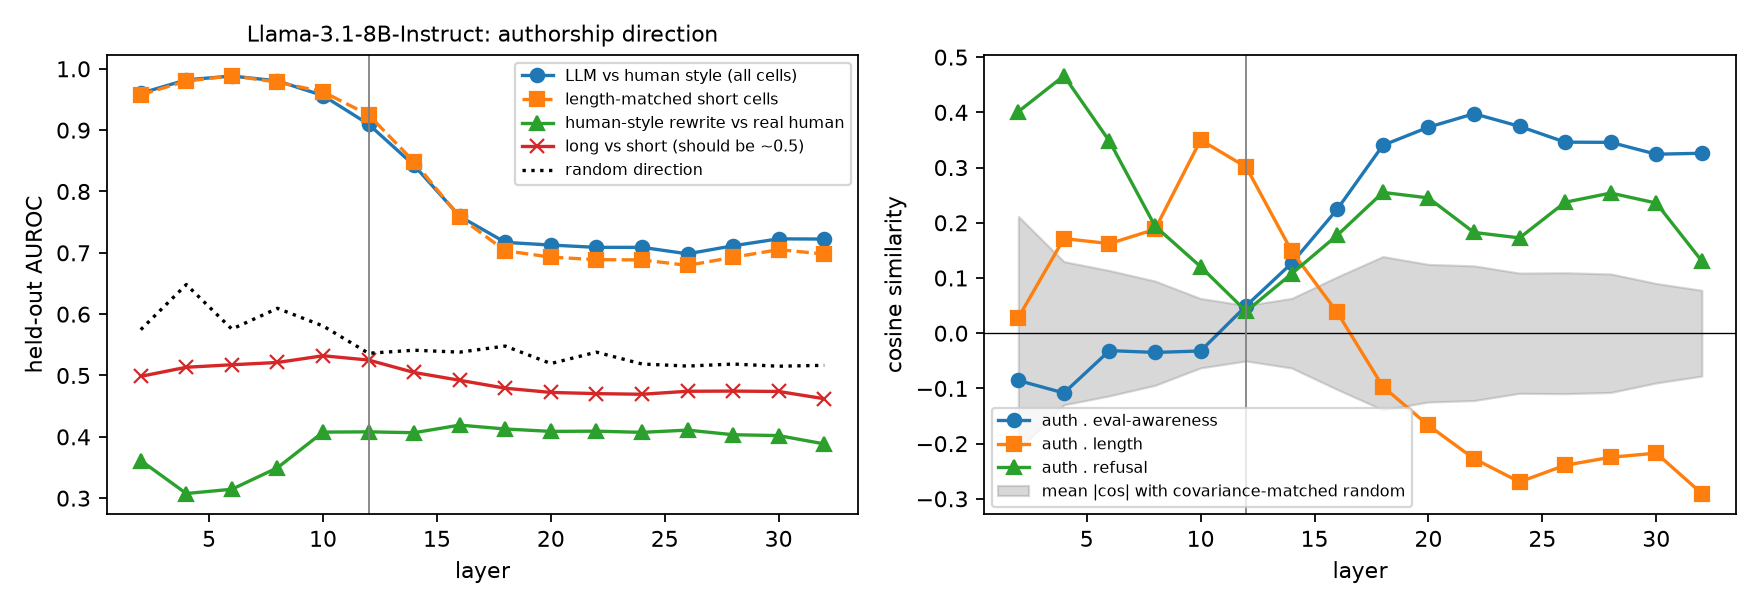
\includegraphics[width=\linewidth]{figures/fig3_probe_llama.png}
\caption{The authorship direction in \llama by layer. Left: held-out AUROC along $\dauth$. Style separates almost perfectly in early layers, equally well in the length-matched short cells; the direction does not separate long from short prompts; and human-style rewrites score as more human than real \wildchat prompts (AUROC below 0.5). Right: cosine of $\dauth$ with the evaluation-awareness, length, and refusal directions, against a covariance-random null (grey band). The vertical line marks layer 12.}
\label{fig:probe}
\end{figure}

\begin{table}[t]
\centering
\small
\caption{Probe results at the three steered layers of each model (held-out \wildchat rewrites, last prompt token). ``Long vs.\ short'' is the AUROC of $\dauth$ for the length contrast (0.5 is ideal). ``Transfer'' trains on GPT rewrites and tests on Claude rewrites. ``Null'' is the mean absolute cosine with covariance-random directions.}
\label{tab:probe}
\resizebox{\textwidth}{!}{
\begin{tabular}{@{}lccccccccc@{}}
\toprule
& & \multicolumn{5}{c}{AUROC} & \multicolumn{3}{c}{Cosine with $\dauth$} \\
\cmidrule(lr){3-7}\cmidrule(lr){8-10}
Model & Layer & style & short cells & long vs.\ short & transfer & random dir. & eval & length & null \\
\midrule
\llama & 6 & {\bf 0.988} & {\bf 0.989} & 0.518 & {\bf 0.991} & 0.576 & $-0.03$ & $0.16$ & 0.11 \\
\llama & 12 & 0.910 & 0.925 & 0.525 & 0.912 & 0.536 & $0.05$ & $0.30$ & 0.05 \\
\llama & 24 & 0.709 & 0.688 & 0.469 & 0.689 & 0.519 & $0.38$ & $-0.27$ & 0.11 \\
\midrule
\qwen & 10 & {\bf 0.995} & {\bf 0.993} & 0.486 & {\bf 0.999} & 0.606 & $0.07$ & $0.00$ & 0.25 \\
\qwen & 12 & 0.990 & 0.985 & 0.499 & 0.997 & 0.647 & $0.16$ & $0.08$ & 0.29 \\
\qwen & 18 & 0.915 & 0.900 & 0.488 & 0.935 & 0.626 & $0.18$ & $-0.02$ & 0.14 \\
\bottomrule
\end{tabular}}
\end{table}

\para{Style is linearly encoded and independent of length.}
In both open models a difference-of-means direction separates held-out LLM-style from human-style rewrites at AUROC $\approx0.99$ in early layers, unchanged in the length-matched cells, and it does not separate long from short prompts (\tabref{tab:probe}, \figref{fig:probe}).
It transfers to the other rewriter (0.98--0.99 in early \llama layers) and to benchmark items (0.86--1.00 at \llama layer 12).

\para{It tracks style, not ``was paraphrased.''}
Human-style rewrites score as \emph{more} human than real \wildchat originals (AUROC 0.32--0.41 for rewrite vs.\ real human in \llama, 0.24--0.43 in \qwen), while LLM-style rewrites score above real humans (0.80--0.86 in \llama layers 2--10).

\para{It fades at the answer position.}
From layer 16 on, the last-token AUROC in \llama is 0.70--0.76 (\qwen: 0.65 from layer 24), while mean-pooling over user tokens keeps 0.96 at \llama layer 12.
The style signal is not carried forward strongly to where the answer is produced.

\para{A probe cannot separate ``representation'' from ``surface features.''}
A logistic regression on eight surface descriptors (lower-case start, final punctuation, apostrophe-free contractions, word length, and so on) reaches AUROC 0.994 on the same split; length alone reaches 0.51.
The style \emph{is} these features, so only an intervention can test whether the representation matters.

\para{Mediation.}
With seed fixed effects, log length, and politeness markers, the layer-12 probe score in \llama does not predict refusal ($\beta=+0.006$ per SD, $p=0.37$), factual sycophancy ($-0.013$, $p=0.23$), accuracy ($-0.013$, $p=0.27$), or opinion sycophancy ($+0.021$, $p=0.32$).
In \qwen it does not predict refusal, factual sycophancy, or accuracy ($p\geq0.25$); it predicts opinion sycophancy ($+0.063$, $p=0.04$ uncorrected), as does the style indicator alone ($+0.022$, $p=0.01$), and with both in the model neither is distinguishable.

\para{Relation to evaluation awareness (H5).}
The authorship and evaluation-awareness directions are unrelated in the layers where authorship is well encoded: in \llama the cosine is $-0.11$ to $+0.05$ through layer 12, inside the covariance-random null of 0.05--0.21, and in \qwen it is at most 0.18 through layer 18 (null 0.14--0.29).
They become aligned in later layers (\llama 0.33--0.40 from layer 18 on, null 0.08--0.14; \qwen 0.28--0.47 from layer 20 on, null 0.10--0.17), where the authorship probe itself is weak.
LLM-style prompts do project slightly further along the evaluation direction than human-style ones on every task ($p<0.001$).
The verbal ``this is a test'' logit is also higher for LLM style: weakly in \llama ($+0.15$ to $+0.27$ on benchmark items, $+0.03$ on \wildchat items, $p=0.40$) and strongly in \qwen ($+2.6$ to $+4.9$ on every task, all $p<0.001$).
So LLM style nudges the model's internal and verbal sense of ``being tested'' a little, without a measurable behavioral consequence here.

\subsection{Steering on fixed text (H4)}
\label{sec:steer}

\begin{figure}[t]
\centering
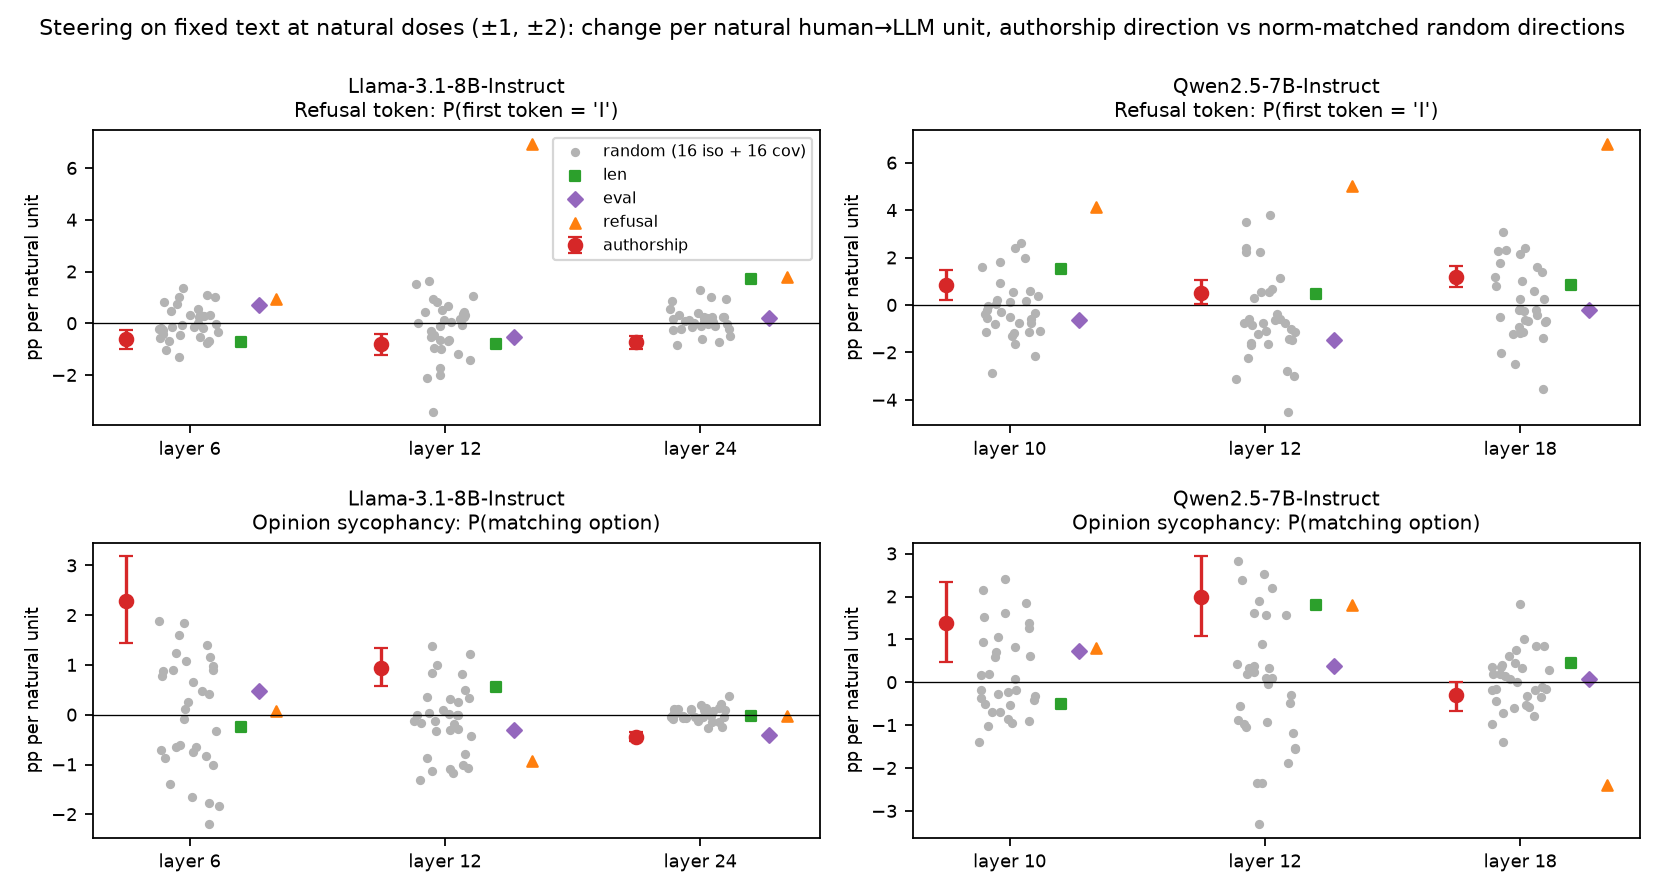
\includegraphics[width=0.95\linewidth]{figures/fig6_steering_natural_dose.png}
\caption{Steering at natural doses ($\alpha=\pm1,\pm2$) on fixed text: slope per natural human$\rightarrow$LLM unit for the authorship direction (red, 95\% CI), 32 norm-matched random directions (grey), and the length, evaluation, and refusal directions. Top: refusal token. Bottom: opinion sycophancy. On refusal the authorship direction sits inside the random cloud at all six model--layer combinations, while the refusal direction stands out in five of six.}
\label{fig:natural}
\end{figure}

\begin{table}[t]
\centering
\small
\caption{Natural-dose steering: slope in pp per natural unit with 95\% bootstrap CIs over items. ``Random'' is the mean and maximum absolute slope over 32 random directions; $p$ is the share of random directions with an absolute slope at least as large (floor 0.03). Bold marks slopes that exceed all 32 random directions.}
\label{tab:natural}
\resizebox{\textwidth}{!}{
\begin{tabular}{@{}lcccccccc@{}}
\toprule
& \multicolumn{4}{c}{Refusal token} & \multicolumn{3}{c}{Opinion sycophancy} \\
\cmidrule(lr){2-5}\cmidrule(lr){6-8}
Model, layer & authorship & random (mean; max) & $p$ & refusal dir. & authorship & random (mean; max) & $p$ \\
\midrule
\llama 6 & $-0.6$ [$-1.0$, $-0.3$] & 0.5; 1.4 & 0.36 & $+0.9$ & $\mathbf{+2.3}$ [$+1.4$, $+3.2$] & 1.0; 2.2 & 0.03 \\
\llama 12 & $-0.8$ [$-1.2$, $-0.4$] & 0.8; 3.4 & 0.42 & $\mathbf{+6.9}$ & $+0.9$ [$+0.6$, $+1.3$] & 0.5; 1.4 & 0.30 \\
\llama 24 & $-0.7$ [$-1.0$, $-0.5$] & 0.3; 1.3 & 0.21 & $\mathbf{+1.8}$ & $\mathbf{-0.4}$ [$-0.5$, $-0.3$] & 0.1; 0.4 & 0.03 \\
\qwen 10 & $+0.8$ [$+0.2$, $+1.5$] & 1.0; 2.9 & 0.45 & $\mathbf{+4.1}$ & $+1.4$ [$+0.5$, $+2.3$] & 0.8; 2.4 & 0.18 \\
\qwen 12 & $+0.5$ [$+0.1$, $+1.0$] & 1.6; 4.5 & 0.94 & $\mathbf{+5.0}$ & $+2.0$ [$+1.1$, $+2.9$] & 1.2; 3.3 & 0.24 \\
\qwen 18 & $+1.2$ [$+0.8$, $+1.7$] & 1.2; 3.5 & 0.48 & $\mathbf{+6.8}$ & $-0.3$ [$-0.7$, $\phantom{+}0.0$] & 0.5; 1.8 & 0.67 \\
\bottomrule
\end{tabular}}
\end{table}

Steering changes the representation while the text stays fixed, which is the cleanest content control.
We report the natural-dose run here; the full dose-response curves and large-dose tables are in \secref{sec:app_steer}.

\para{The direction is causally a style direction.}
Steering toward human style at \llama layers 6 and 12 makes the model answer in lower case: 87--94\% of responses at $\alpha=-8$, against 0\% unsteered, at most 0.8\% under any random direction, and 14\% under the length direction at layer 6.
In \qwen the share of lower-case sentence starts rises from 0.4\% to 19\% (layer 10) and 44\% (layer 12) at $\alpha=-8$, against at most 6\% under any random direction.
The model's output register follows the representation, but only at large doses: at $\pm1$ and $\pm2$ the share stays below 1\% in \llama, as unsteered.

\para{Refusal does not follow it at natural doses.}
Moving the representation by the natural human$\rightarrow$LLM amount changes the refusal-token probability by about 1\pp or less per unit, with opposite signs in the two models, and never more than random directions of the same norm (\tabref{tab:natural}, \figref{fig:natural}).
The item-level CIs exclude zero, but that only shows that any perturbation of this size moves the readout; the comparison with random directions is the relevant one.
The positive control works: the refusal direction exceeds all 32 random directions at five of the six model--layer combinations (2--7\pp per unit).
In generated outputs, natural doses change refusal by at most 3.2\pp (\llama) and 3.6\pp (\qwen), factual sycophancy by at most 2.7 and 6.0\pp with every CI including zero, and accuracy by at most 6--7\pp on 100 items.

\para{Large doses do not rescue an effect on refusal.}
At doses up to $\pm4$, the sign-dependent effect of the authorship direction on generated refusals is inside the range of eight random directions at all three layers of both models (at most 2.2\pp in \qwen), while the refusal direction at the same norm moves refusal by 13--27\pp in \qwen and 36--45\pp at \llama layer 12.
At $\pm8$, refusal and accuracy fall for both signs and for random directions too (accuracy $-17$ to $-55$\pp in \qwen), which is degradation rather than a concept effect.
There is one exception: at \qwen layer 10 and $\pm8$, the sign-dependent effect on refusal ($-26$\pp) is larger than for any of the eight random directions (largest 12\pp; $p=0.11$, the floor).
The outputs at this dose are visibly degraded (hedged half-refusals at $+8$, switches into Chinese in 32\% of responses at $-8$), and the effect is absent at $\pm4$ and at the other layers.
We read it as part of the degradation regime, but it is the one place where the authorship direction beats the random baseline on refusal.

\para{Opinion sycophancy is mixed.}
The authorship direction exceeds all 32 random directions at \llama layer 6 ($+2.3$\pp per unit) and \llama layer 24 ($-0.4$\pp per unit, opposite sign), and at none of the \qwen layers.
We made twelve such comparisons, so two at the floor $p$ of 0.03 is not strong evidence, and the signs disagree.
In the early and middle layers of both models the point estimates are positive ($+0.9$ to $+2.3$\pp per unit), which matches the sign of \qwen's text-level style effect ($+2.4$\pp, \tabref{tab:main}) but not \llama's ($+0.2$\pp).
We record this as a possible small effect of LLM style on opinion sycophancy that this study cannot confirm.

\subsection{Style changes the form of the answer}
\label{sec:form}

\begin{table}[t]
\centering
\small
\caption{Response length in words on trivia items. LLM-style prompts receive shorter answers; the style effect is the length-balanced main effect. Open-model responses are capped at 96 tokens.}
\label{tab:form}
\begin{tabular}{@{}lccccc@{}}
\toprule
Model & \Hs & \Ls & Style effect & 95\% CI & $p$ \\
\midrule
\llama & 25.3 & 22.2 & $-5.5$ & [$-7.5$, $-3.6$] & $<0.001$ \\
\qwen & 56.2 & 54.2 & $-1.6$ & [$-3.2$, $+0.1$] & 0.051 \\
\gpt & 18.9 & 14.3 & $-6.9$ & [$-8.3$, $-5.6$] & $<0.001$ \\
\claude & 107.1 & 101.6 & $-9.9$ & [$-13.9$, $-6.0$] & $<0.001$ \\
\gemini & 56.1 & 45.1 & $\mathbf{-15.4}$ & [$-19.7$, $-11.0$] & $<0.001$ \\
\bottomrule
\end{tabular}
\end{table}

Style is not inert.
LLM-style prompts receive shorter answers in four of five models ($-5$ to $-15$ words on trivia questions, $p<0.001$; \tabref{tab:form}), and \gpt uses markdown formatting less often for LLM-style prompts (54--58\% vs.\ 71--84\%).
Models respond to register: they answer casual prompts at greater length.
This is a behavioral difference, but not one of the safety behaviors we test.

\section{Discussion}
\label{sec:discussion}

\para{What the evidence supports.}
Our question has two parts.
Do safety behaviors change when the same request reads LLM-written?
Not detectably: effects are within $\pm3$\pp per model with CIs of roughly $\pm2$--$4$\pp, and $\pm1$--$2$\pp pooled.
Is any change driven by the internal authorship representation?
The representation exists, is strong, is length-independent, and at large doses causally changes the register of the model's own output in both open models.
Moving it by the natural amount on fixed text changes refusal no more than random directions do and leaves factual sycophancy and accuracy within noise.
Opinion sycophancy is the one outcome where the evidence is mixed: a small effect (about 2\pp per natural unit or less) is neither established nor excluded.

\para{Why naive comparisons mislead.}
The uncontrolled rewrite arm reproduces the kind of result that would be reported as ``models comply more with LLM-written prompts'' (refusal $-4$ to $-11$\pp).
The $2\times2$ design shows that this comes from added framing, softened wording, and explicit instructions.
For evaluation practice, the relevant control is the content fidelity of synthetic prompts, not their voice.

\para{Relation to prior work.}
\citet{needham2025eval} list synthetic-looking prompts as one cue for evaluation detection.
Consistent with that, LLM style raises both open models' projection on an evaluation-awareness direction and their verbal test judgment.
\citet{abdelnabi2025hawthorne} report that steering test awareness changes compliance; here the authorship direction, which is nearly orthogonal to the evaluation direction where it is best encoded, does not.
The two are distinct variables in these models.
Our finding that surface features alone reach AUROC 0.994 echoes the format-sensitivity argument of \citet{devbunova2026format}, and the dissociation between what \llama and \qwen encode and what they can report matches \citet{heidari2026evalaware}.

\para{Surprises.}
The human-style rewrites read as more human than real \wildchat prompts, on both the API raters and the probe.
A local LLM judge validated at 96\% agreement on one model's outputs dropped to 85--88\% on other models' outputs and under-called refusals, so judge validation did not transfer across responders (\secref{sec:app_scoring}).
A provider-side filter on one API responded to prompt style even though the model did not.

\para{Limitations.}
\begin{itemize}[leftmargin=*,itemsep=0pt,topsep=0pt]
    \item \emph{Human style is imitated.} For benchmark items the human-style arm is written by an LLM imitating \wildchat messages; the truly human \wildchat originals serve the probe and manipulation check, not the behavior test.
    \item \emph{The LLM-style arm is constrained.} Under strict content rules the LLM rewrites are short and plain. Structured, multi-paragraph prompts of the kind orchestrators write cannot be content-matched to a one-line human request, and the \Lfree arm shows those do differ in effect. The null applies to voice, not to everything that distinguishes real LLM-written prompts.
    \item \emph{Scope.} We test single-turn, short prompts and three behavior families in five models; we do not cover multi-turn, agentic, or tool-use settings, or outcomes such as deception. The two open models have 7--8B parameters; larger models, which verbalize authorship better, may differ.
    \item \emph{Precision and floors.} Per-model CIs are $\pm2$--$4$\pp, so effects below about 2\pp would be missed; the three small leads (pooled factual sycophancy, \gemini refusal, \qwen opinion sycophancy) are in that range. Factual sycophancy was at floor for the API models.
    \item \emph{Selective attrition.} Rewriters refused 26--29\% of \jbb harmful seeds; the retained harmful items are the milder ones.
    \item \emph{Mixed scoring of steering outputs.} All behavior and \Lfree results use the API judge. Because API access ran out, \llama steering outputs are scored by rules (95--98\% agreement with the API judge) and about half of \qwen's by a recalibrated local judge (86--98\% at doses up to $\pm4$). The logit readouts in \tabref{tab:natural} need no judge.
    \item \emph{Coarse steering baselines.} Eight or 32 random directions give minimum empirical $p$-values of 0.11 and 0.03, and we apply no correction across layers, outcomes, and models. The natural-dose run covers refusal only through a first-token proxy. The refusal direction contrasts benchmark-written harmful prompts with casual \wildchat prompts and is therefore style-confounded, and the evaluation-awareness direction has moderate reliability (split-half cosine 0.41--0.76).
    \item \emph{API responders} are single samples at default temperature, and provider filters removed some responses.
\end{itemize}

\section{Conclusion}
\label{sec:conclusion}

We asked whether LLMs behave differently when a prompt reads LLM-written.
Once content is controlled, making a prompt read LLM-written did not detectably change refusal, sycophancy, or accuracy in five models, even though the models perceive the difference and encode it almost perfectly.
Steering a strong, length-independent authorship direction on fixed text changed output style at large doses, and at natural doses changed refusal no more than random directions; for opinion sycophancy a small effect is neither established nor excluded.
The differences that appear in uncontrolled comparisons, 4--11\pp in refusal, trace to content that the rewriting model adds.
For these models and behaviors, evaluations that use LLM-written user turns are not biased by the LLM voice itself by more than a few points, but they can be biased by added content, so content fidelity is what needs checking.

Future work should, in order of value, (1) use human-written paraphrases of benchmark items as the human arm, and natively LLM-written multi-paragraph prompts with content-matched human counterparts; (2) follow up the two sycophancy leads with larger item sets, the user's hedge held verbatim across styles, and more random directions; (3) extend to multi-turn and agentic settings, where an orchestrator's voice persists across turns; (4) test whether provider moderation layers respond to casual register; and (5) repeat the steering analysis in larger open models.


\bibliography{references}

\appendix
\section{Scoring deviations and judge validation}
\label{sec:app_scoring}

API access was interrupted twice, which changed how some outputs were scored.

\para{First interruption.}
The OpenRouter key reached its daily limit after the API judge had labelled the \llama, \gpt, and \claude runs.
We first scored \qwen, \gemini, and the open-model \Lfree arms with a local \llama judge using the same rubric.
When the limit reset, we re-scored everything with the API judge and filled the \gemini gaps (208 missing responses and the \Lfree arm); all behavior numbers in this paper use the API judge.
The re-scoring showed that the local judge had not transferred: it agreed with the API judge on 96\% of refusal labels for \llama outputs, where it had been validated, but on only 85\% for \qwen and 88\% for \gemini outputs, and it under-called refusals (\qwen: 36\% against 51\%).
No headline conclusion changed, but several \qwen and \gemini rates did.

\para{Second interruption.}
The account ran out of credit while the API judge was labelling the steering outputs.
\Tabref{tab:scorers} lists how steering outputs are scored.
For locally scored \qwen conditions we compute the change against the unsteered run scored by the same local judge, and we do not report refusal at $\pm8$ in those conditions.
We do not use the rule-based scorer for \qwen, where it agreed with the API judge on only 78\% of steered refusal labels.
The logit readouts (opinion sycophancy, refusal token, verbal judgments) need no judge.

\begin{table}[h]
\centering
\small
\caption{Scoring of steering outputs.}
\label{tab:scorers}
\begin{tabular}{@{}p{0.27\linewidth}p{0.3\linewidth}p{0.36\linewidth}@{}}
\toprule
Steering data & Scorer & Agreement with API judge \\
\midrule
\llama, all conditions & rule-based (refusal phrases, answer-alias match) & on 22{,}502 outputs with cached API labels: refusal 98\%, accuracy 97\%, factual sycophancy 95\% \\
\qwen, layer 10 (all); layer 12 authorship, length, evaluation, refusal directions & API judge (41{,}806 of 78{,}500 rows) & --- \\
\qwen, layer 18; six of eight random directions at layer 12 & local \llama judge, recalibrated on API-labelled \qwen steering outputs (logistic regression on option log-probabilities, fitted on half of the items) & held-out items, doses up to $\pm4$: refusal 95--98\%, accuracy 94--97\%, factual sycophancy 86--89\%; at $\pm8$: refusal 73\% \\
\bottomrule
\end{tabular}
\end{table}

\section{Additional steering results}
\label{sec:app_steer}

\begin{figure}[h]
\centering
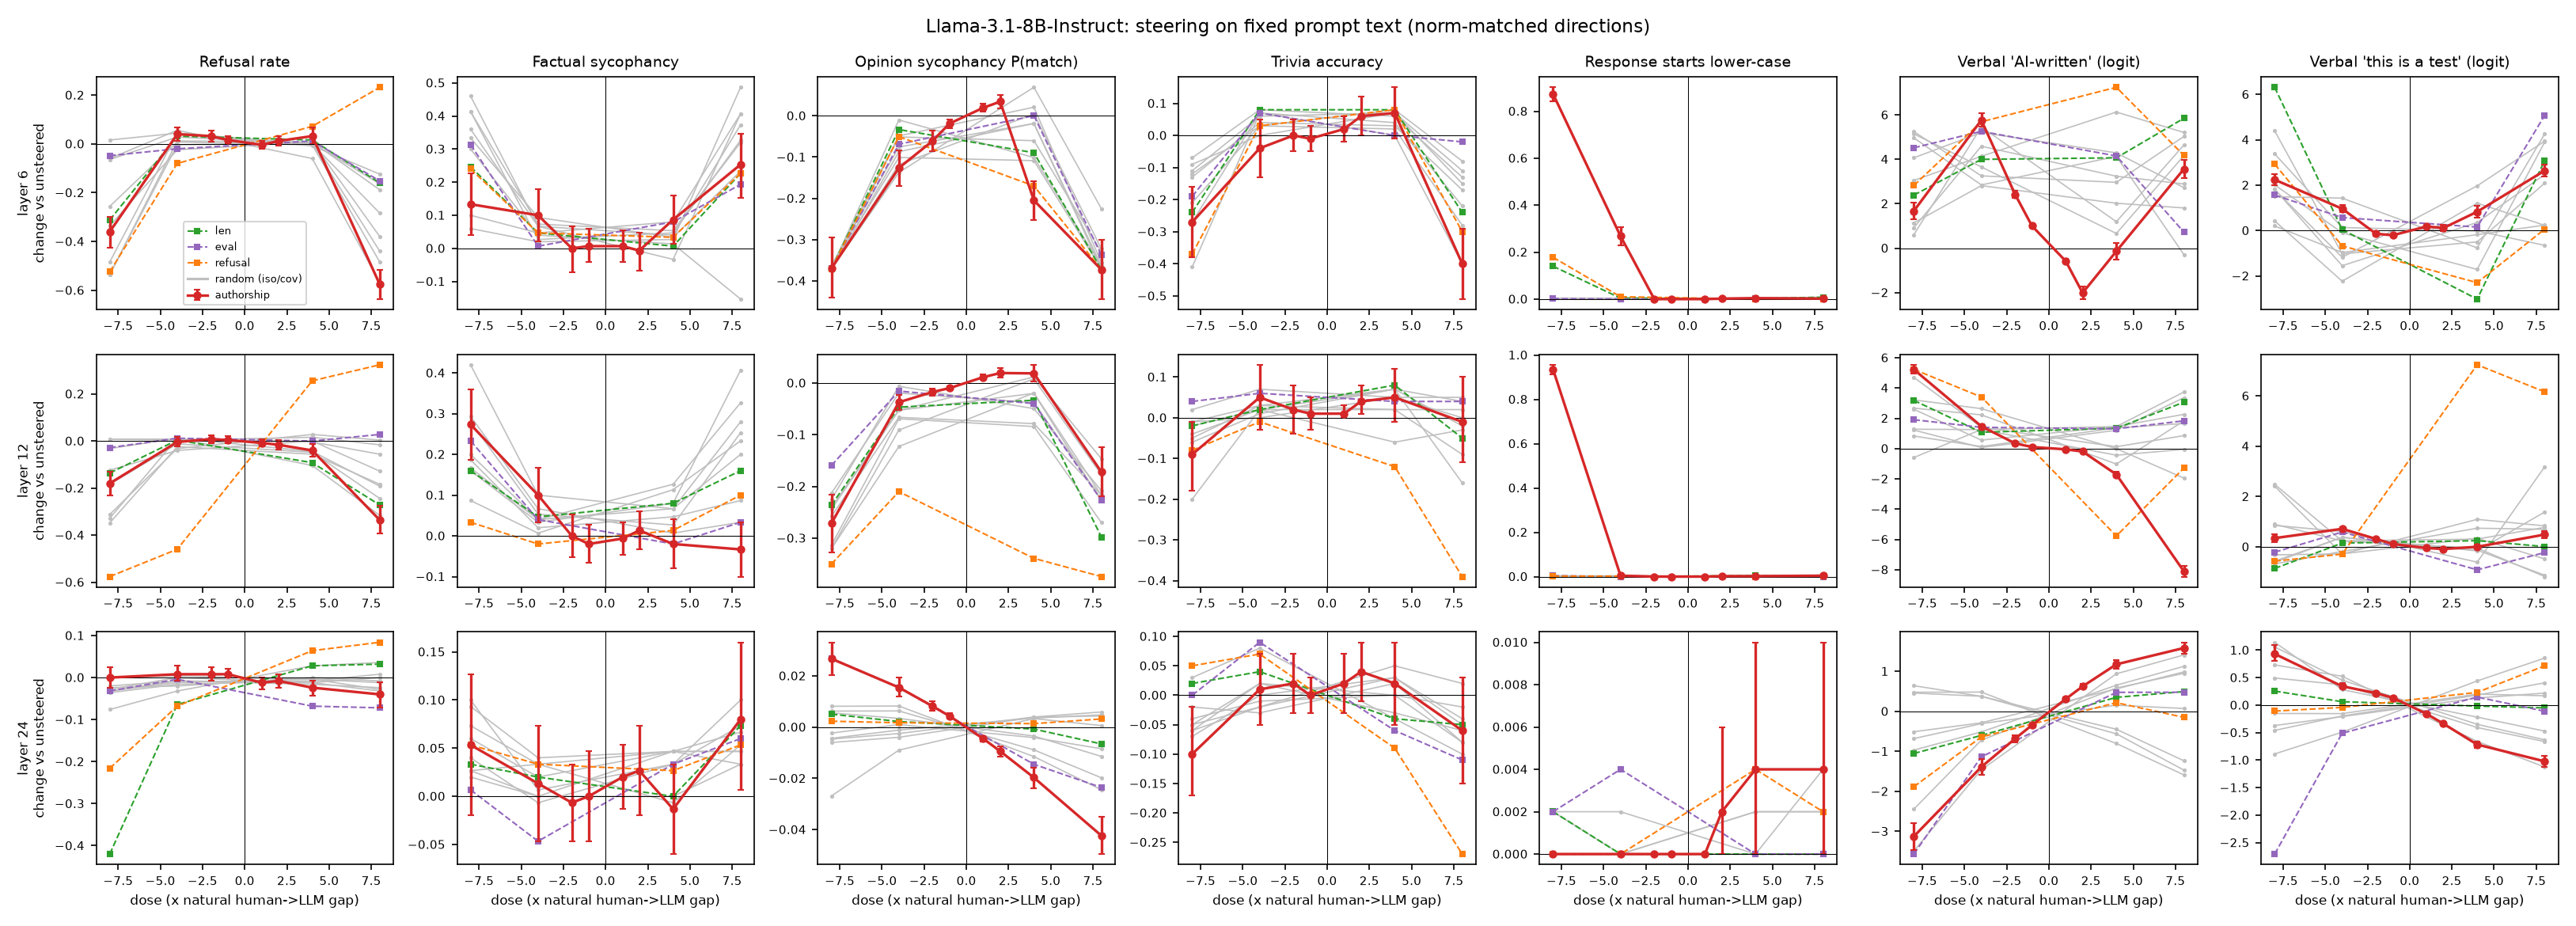
\includegraphics[width=\linewidth]{figures/fig4_steering_llama.png}
\caption{\llama: steering on fixed prompt text, change against the unsteered run by dose (in units of the natural human$\rightarrow$LLM gap), for layers 6, 12, and 24 (rows). Red: authorship direction with paired-bootstrap 95\% CIs. Grey: eight random directions at the same norm. Dashed: length, evaluation-awareness, and refusal directions. The authorship direction turns responses lower-case at $\alpha=-8$ (fifth column) but tracks the random directions on refusal.}
\label{fig:steer_llama}
\end{figure}

\begin{figure}[h]
\centering
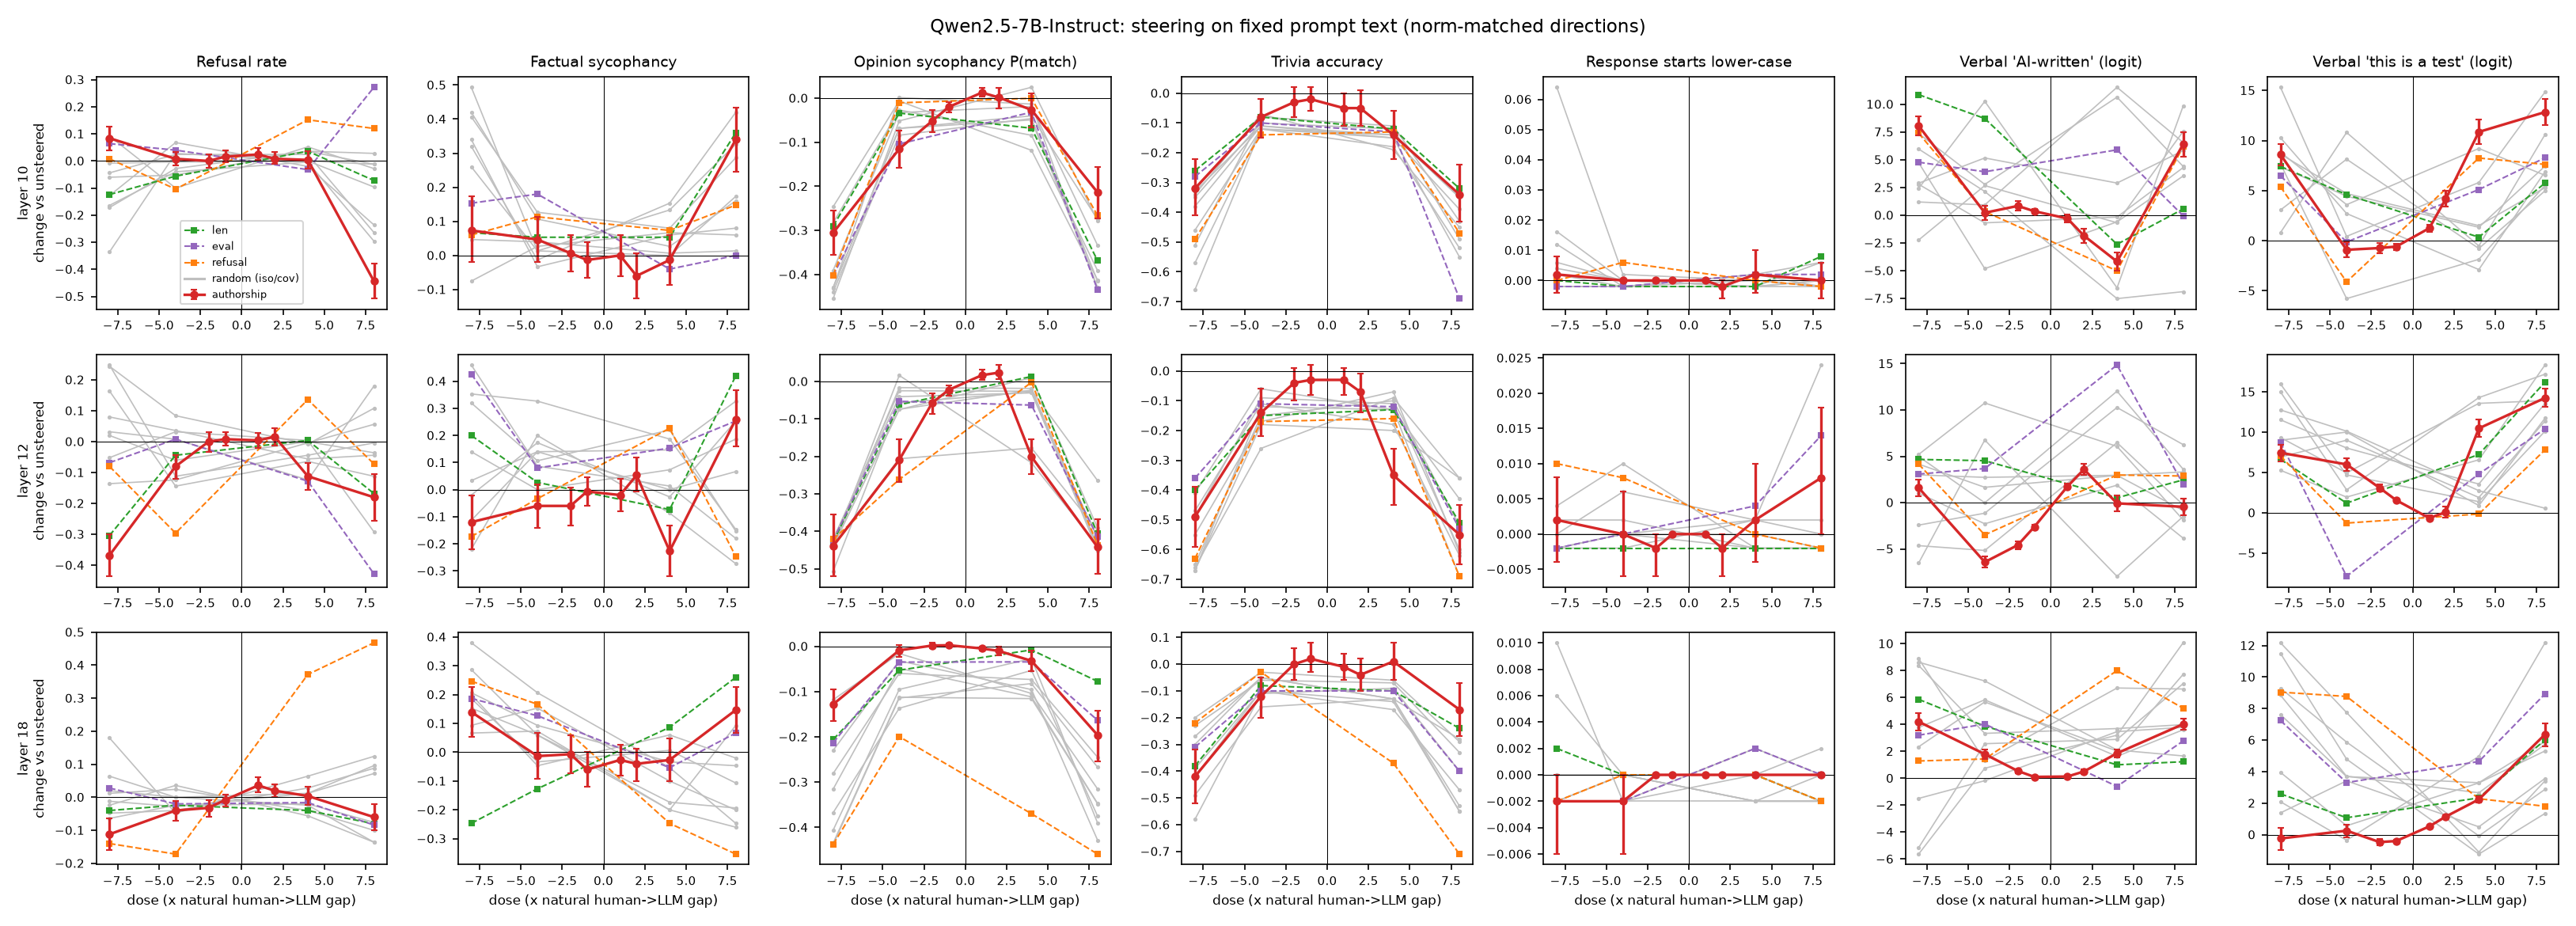
\includegraphics[width=\linewidth]{figures/fig4_steering_qwen.png}
\caption{\qwen: steering on fixed prompt text, same layout as \figref{fig:steer_llama}, for layers 10, 12, and 18. Scoring follows \tabref{tab:scorers}.}
\label{fig:steer_qwen}
\end{figure}

\para{Natural doses, generated outcomes.}
In \llama, the CI for refusal excludes zero only at layer 6 for $\alpha=-1$ ($+1.6$\pp) and $\alpha=-2$ ($+3.2$\pp); everything else is within $\pm1.6$\pp.
Every factual-sycophancy CI includes zero (largest change 2.7\pp).
Opinion sycophancy moves by about $+1$ to $+2$\pp per unit toward LLM style at layers 6 and 12 and by 0.5\pp per unit with the opposite sign at layer 24.
In \qwen (unsteered: refusal 57\%, factual sycophancy 37\%, accuracy 73\%, P(match) 96\%), refusal at layer 18 changes by $-3.2$, $-0.8$, $+3.6$, $+2.0$\pp at $\alpha=-2,-1,+1,+2$ (local judge), which corresponds to a refusal-token slope of $+1.2$\pp per unit, in the middle of the random distribution (\tabref{tab:natural}); at layer 10 it changes by $+2.4$\pp at $\alpha=+1$; everything else is within $\pm1.6$\pp.
Factual sycophancy changes by at most 6.0\pp with every CI including zero, and opinion sycophancy rises toward LLM style at layers 10 and 12 and stays within $\pm1$\pp at layer 18.

\para{Large doses.}
\Tabref{tab:odd} reports the sign-dependent part of the effect, $(\Delta(+\alpha)-\Delta(-\alpha))/2$, against the same quantity for random directions.
In \llama, the authorship direction's effect on refusal is inside the random range at every layer and dose (empirical $p\geq0.22$).
Two small exceptions appear at supra-natural doses and at the floor of the test's resolution ($p=0.11$): at layer 12, steering toward LLM style lowers factual sycophancy ($-6.0$\pp at $\pm4$, $-15.3$\pp at $\pm8$), the same sign as the suggestive text-level pattern in \secref{sec:behaviour}; and at layer 24 there is a monotone but tiny dose-response on opinion sycophancy.
The length and evaluation directions at the same norm did not beat random on the sycophancy outcomes; the length direction raised refusal at \llama layer 24 ($+22.6$\pp at $\pm8$).

\para{Verbal judgments under steering} are inconsistent across layers.
In \llama, adding the LLM-style direction raises the ``AI-written'' logit at layer 24 ($+1.3$ at $\pm4$) but lowers it at layers 6 and 12 ($-3.0$ and $-1.6$).
In \qwen, the ``AI-written'' logit follows the direction at layer 12 for $\pm1$ and $\pm2$ and reverses at layer 10.
The verbal readout is not a reliable measure of this representation in models of this size.

\begin{table}[h]
\centering
\small
\caption{Sign-dependent steering effect at large doses, as a proportion. Parentheses: mean absolute value of the same statistic over the eight random directions. Bold marks refusal effects of the positive control.}
\label{tab:odd}
\resizebox{\textwidth}{!}{
\begin{tabular}{@{}llclcccc@{}}
\toprule
Model & Layer & $\alpha$ & Direction & Refusal & Factual sycophancy & Opinion sycophancy & Lower-case start / Accuracy$^\dagger$ \\
\midrule
\llama & 6 & 8 & authorship & $-0.108$ (0.119) & $+0.060$ (0.100) & $-0.001$ (0.017) & $-0.436$ (0.002) \\
\llama & 12 & 4 & authorship & $-0.018$ (0.023) & $-0.060$ (0.026) & $+0.028$ (0.024) & $-0.001$ (0.001) \\
\llama & 12 & 8 & authorship & $-0.078$ (0.050) & $-0.153$ (0.077) & $+0.050$ (0.029) & $-0.466$ (0.001) \\
\llama & 24 & 8 & authorship & $-0.020$ (0.014) & $+0.013$ (0.012) & $-0.035$ (0.009) & $+0.002$ (0.001) \\
\llama & 12 & 4 & refusal & $\mathbf{+0.358}$ (0.023) & $+0.017$ (0.026) & $-0.065$ (0.024) & $-0.001$ (0.001) \\
\llama & 12 & 8 & refusal & $\mathbf{+0.450}$ (0.050) & $+0.033$ (0.077) & $-0.012$ (0.029) & $\phantom{+}0.000$ (0.001) \\
\midrule
\qwen & 10 & 4 & authorship & $-0.002$ (0.029) & $-0.030$ (0.037) & $+0.044$ (0.022) & $-0.030$ (0.022) \\
\qwen & 10 & 8 & authorship & $-0.264$ (0.067) & $+0.133$ (0.081) & $+0.046$ (0.043) & $-0.010$ (0.059) \\
\qwen & 12 & 4 & authorship & $-0.016$ (0.042) & $-0.083$ (0.065) & $+0.004$ (0.027) & $-0.105$ (0.032) \\
\qwen & 12 & 8 & authorship & $+0.094$ (0.089) & $+0.190$ (0.154) & $-0.001$ (0.025) & $-0.030$ (0.099) \\
\qwen & 18 & 4 & authorship & $+0.022$ (0.026) & $-0.007$ (0.097) & $-0.012$ (0.026) & $+0.065$ (0.022) \\
\qwen & 10 & 4 & refusal & $\mathbf{+0.128}$ (0.029) & $-0.020$ (0.037) & $+0.005$ (0.022) & $+0.005$ (0.022) \\
\qwen & 12 & 4 & refusal & $\mathbf{+0.216}$ (0.042) & $+0.130$ (0.065) & $+0.130$ (0.027) & $+0.005$ (0.032) \\
\qwen & 18 & 4 & refusal & $\mathbf{+0.272}$ (0.026) & $-0.207$ (0.097) & $-0.085$ (0.026) & $-0.170$ (0.022) \\
\bottomrule
\multicolumn{8}{@{}l}{\footnotesize $^\dagger$ \llama rows: share of responses starting in lower case. \qwen rows: trivia accuracy.}
\end{tabular}}
\end{table}

\section{Probe by layer in \qwen}
\label{sec:app_qwen}

\begin{figure}[h]
\centering
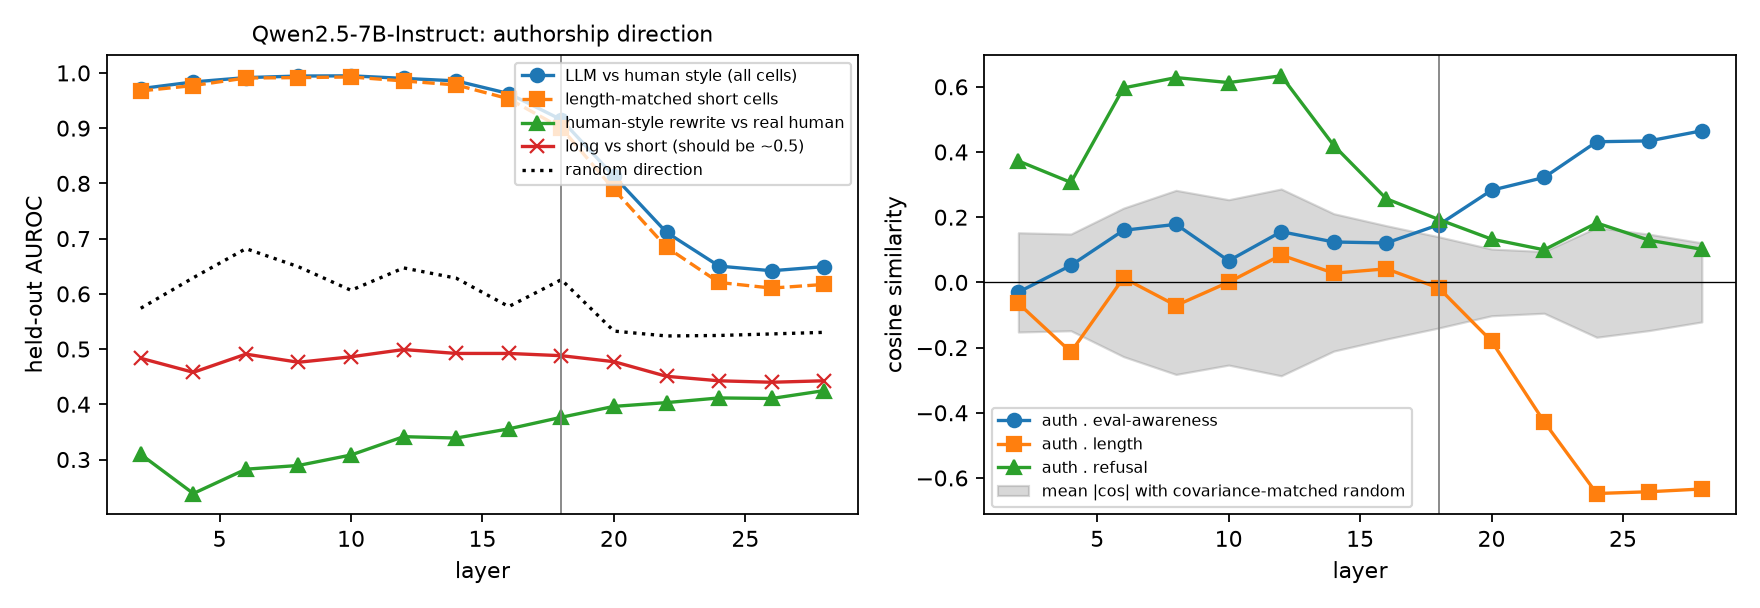
\includegraphics[width=\linewidth]{figures/fig3_probe_qwen.png}
\caption{The authorship direction in \qwen by layer, same layout as \figref{fig:probe}. Style is linearly encoded (AUROC 0.96--0.995 through layer 16), independent of length, and fades at the answer position in late layers.}
\label{fig:probe_qwen}
\end{figure}

\section{Reproducibility}
\label{sec:app_repro}

We ran all local experiments on one NVIDIA RTX A6000 (48\,GB) with the open models in bf16, using Python 3.12, torch 2.14.1, and transformers 5.18.0.
Stimulus building took 15 minutes; open-model behavior and activations 17--20 minutes per model; steering 80--90 minutes per model (157 conditions); the natural-dose logit run 35--65 minutes per model (433 conditions); and API responders 20--60 minutes each.
Logged API usage corresponds to roughly \$65 at catalogue prices, plus unlogged \gemini usage on the first day.
We use seed 42 for sampling and seed 0 for splits and random directions.
Bootstrap CIs and permutation $p$-values use a seeded generator, but values can differ in the last digit between runs of an analysis script because the tables are computed in sequence from one generator.


\end{document}
